\documentclass{article}
\usepackage{amsmath,amssymb,amsthm,kotex,mdframed,paralist}
\newcounter{num}
%\newcommand{\defi}[1]
%{\bigskip\noindent\refstepcounter{num}\textbf{정의 \arabic{num}) #1}\par}
\newcommand{\theo}[1]
{\bigskip\noindent\refstepcounter{num}\textbf{정리 \arabic{num}) #1}\par}
\newcommand{\exam}[1]
{\bigskip\noindent\refstepcounter{num}\textbf{예시 \arabic{num}) #1}\par}
\newcommand{\prob}[1]
{\bigskip\noindent\refstepcounter{num}\textbf{문제 \arabic{num}) #1}\par}
\newcommand{\summ}[1]
{\bigskip\noindent\refstepcounter{num}\textbf{요약 \arabic{num}) #1}\par}

\newcommand{\pb}[1]%\Phantom + fBox
{\fbox{\phantom{\ensuremath{#1}}}}


\renewcommand{\figurename}{그림}
%\renewcommand{\proofname}{증명)}
\newcommand{\sol}{\par\bigskip\noindent{\bfseries풀이)}\par}
\newcommand{\ans}[1]{{\raggedleft\textbf{답 : }#1\par}}

%%%%
\begin{document}

\title{준영 : 02 무리함수의 그래프}
\author{}
\date{\today}
\maketitle
\tableofcontents
\newpage

%%
\section{평행이동과 대칭이동 복습}

\begin{figure}[h!]
\centering
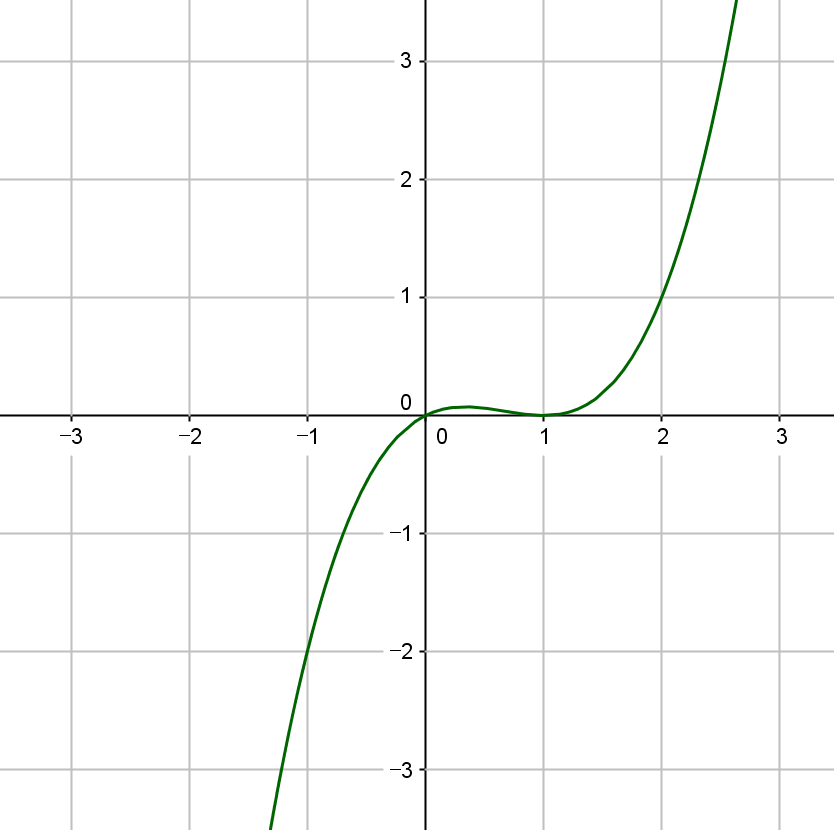
\includegraphics[width=0.49\textwidth]{review_1_1}
\end{figure}

함수 \(y=f(x)\)의 그래프가 위 그림과 같을 때, 이 그래프를 사용하여 여러 가지 함수의 그래프들을 그릴 수 있다.

\bigskip\par\noindent
{\footnotesize
\begin{tabular}{p{0.49\textwidth}|p{0.49\textwidth}}
\hline
\raisebox{-.5\height}{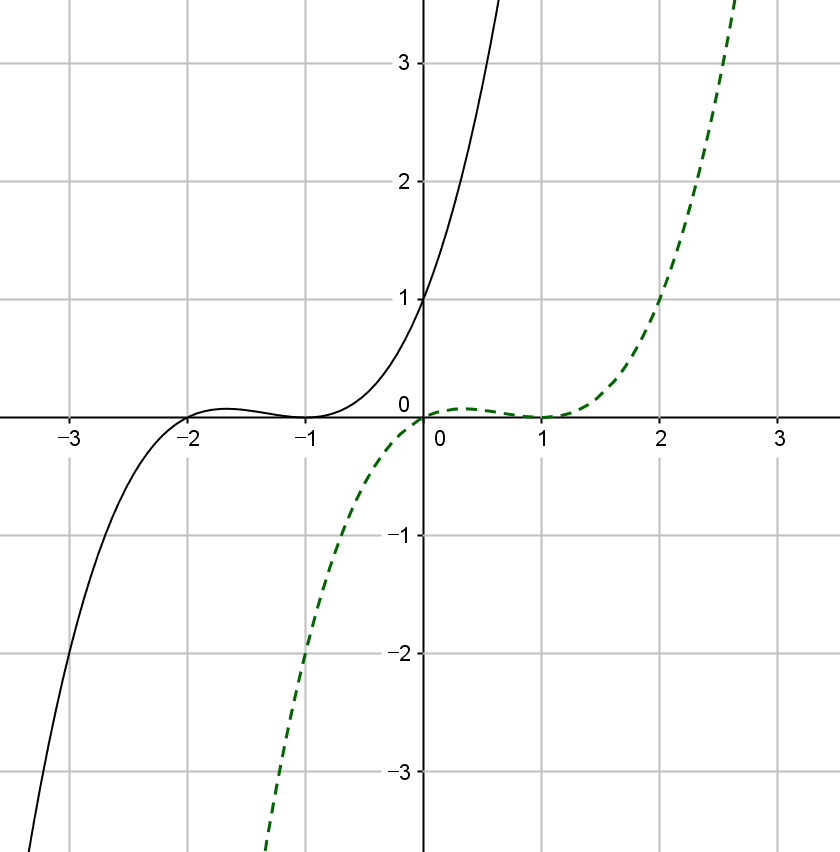
\includegraphics[width=0.49\textwidth]{review_1_2}}
&\raisebox{-.5\height}{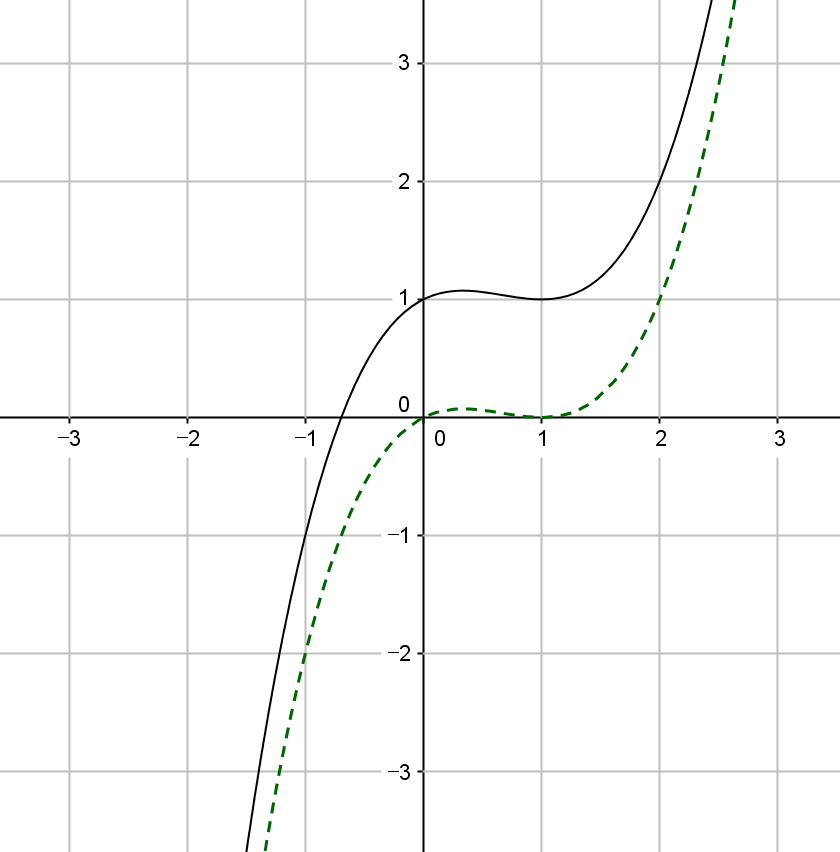
\includegraphics[width=0.49\textwidth]{review_1_3}}
\\\hline
\(y=f(x+2)\)&\(y=f(x)+1\)
\\
\(x\) 대신에 \(x+2\)를 대입&\(y\) 대신에 \(y-1\)을 대입
\\
\(x\)축 방향으로 \(-2\)만큼 평행이동&\(y\)축 방향으로 \(1\)만큼 평행이동
\\\hline
\end{tabular}
}

\par\noindent
{\footnotesize
\begin{tabular}{p{0.49\textwidth}|p{0.49\textwidth}}
\hline
\raisebox{-.5\height}{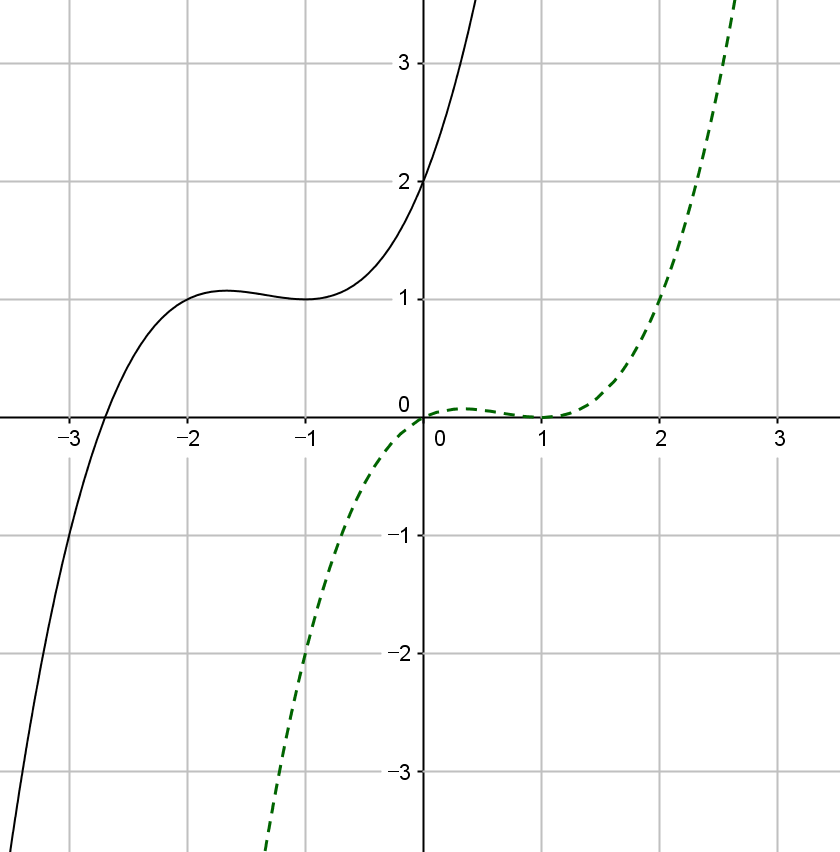
\includegraphics[width=0.49\textwidth]{review_1_4}}
&\raisebox{-.5\height}{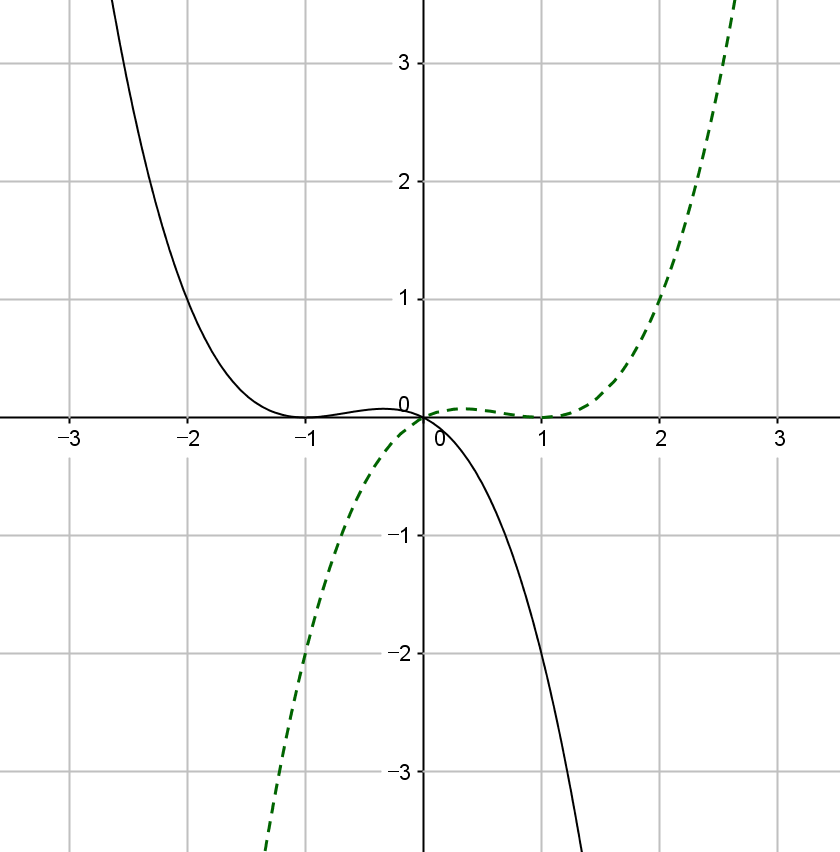
\includegraphics[width=0.49\textwidth]{review_1_5}}
\\\hline
\(y=f(x+2)+1\)&\(y=f(-x)\)
\\
\(x\), \(y\) 대신에 각각 \(x+2\),  \(y-1\)을 대입
& \(x\) 대신에 \(-x\)를 대입
\\
\(x\)축, \(y\)축 방향으로 \(-2\), \(1\)만큼 평행이동
&\(y\)축을 중심으로 대칭이동
\\\hline
\end{tabular}
}

\par\noindent
{\footnotesize
\begin{tabular}{p{0.49\textwidth}|p{0.49\textwidth}}
\raisebox{-.5\height}{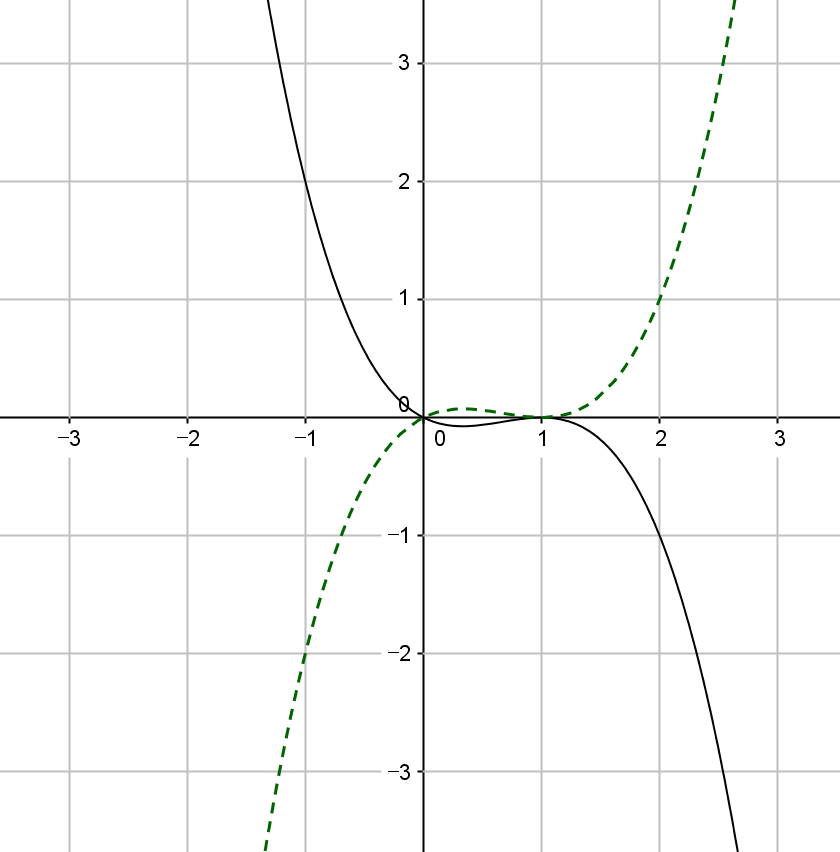
\includegraphics[width=0.49\textwidth]{review_1_6}}
&\raisebox{-.5\height}{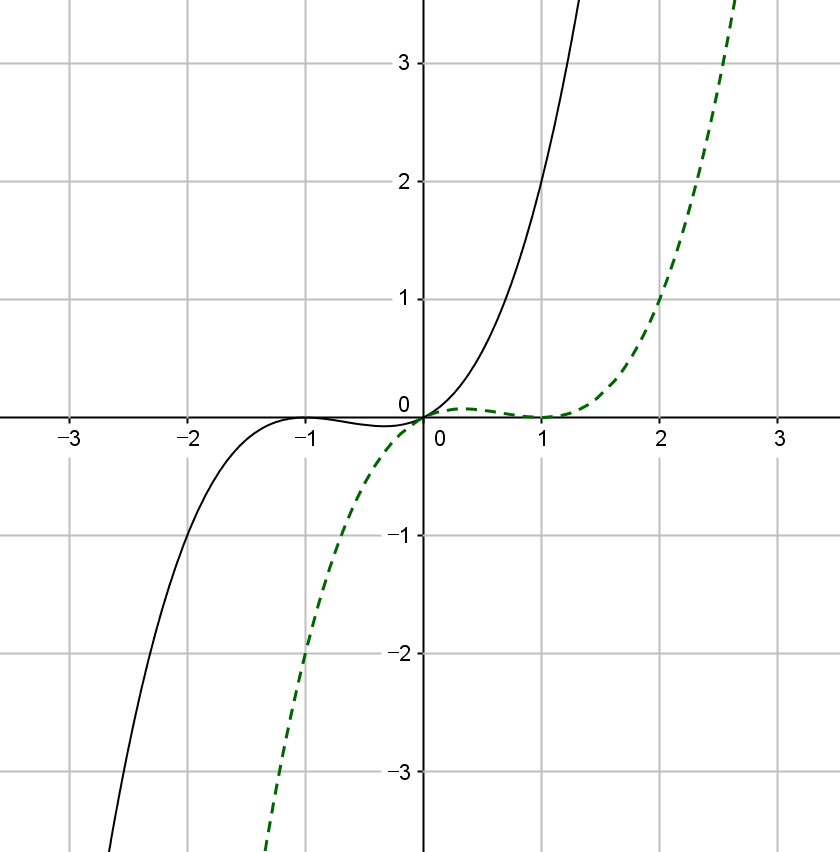
\includegraphics[width=0.49\textwidth]{review_1_7}}
\\\hline
\(y=-f(x)\)&\(y=-f(-x)\)
\\
\(y\) 대신에 \(-y\)를 대입
& \(x\), \(y\) 대신에 각각 \(-x\), \(-y\)를 대입
\\
\(x\)축을 중심으로 대칭이동
&원점을 중심으로 대칭이동
\\\hline
\end{tabular}
}

\clearpage

%
\prob{}
\begin{figure}[h!]
\centering
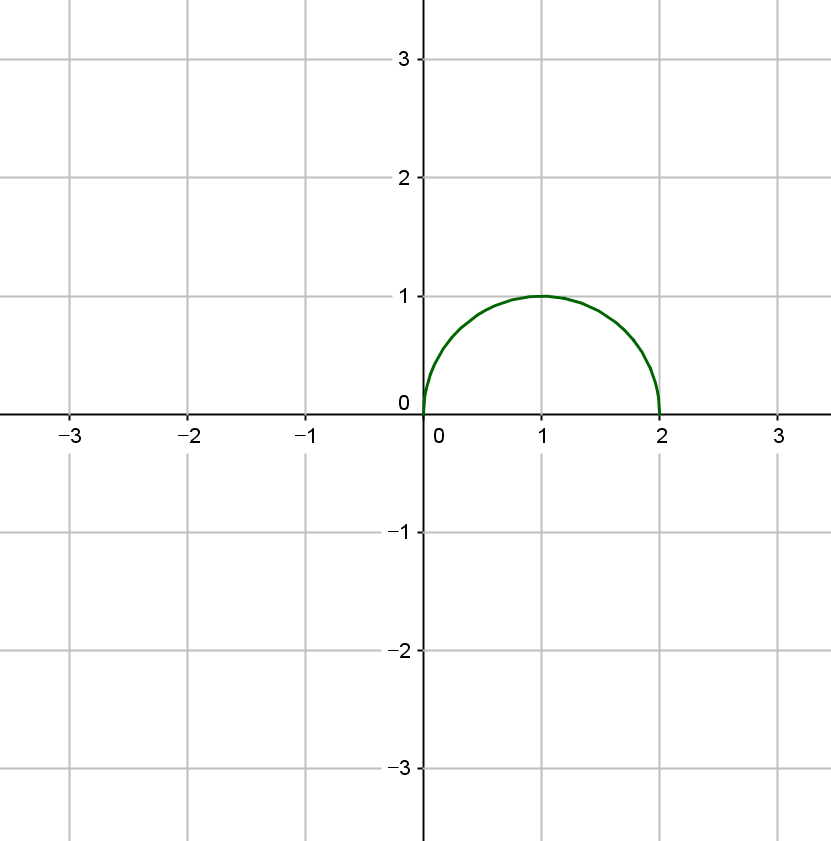
\includegraphics[width=0.49\textwidth]{review_2_1}
\end{figure}
함수 \(y=f(x)\)의 그래프가 위 그림과 같을 때, 다음 함수들의 그래프들을 그리시오.

\bigskip\par\noindent
{\footnotesize
\begin{tabular}{p{0.49\textwidth}|p{0.49\textwidth}}
\hline
\raisebox{-.5\height}{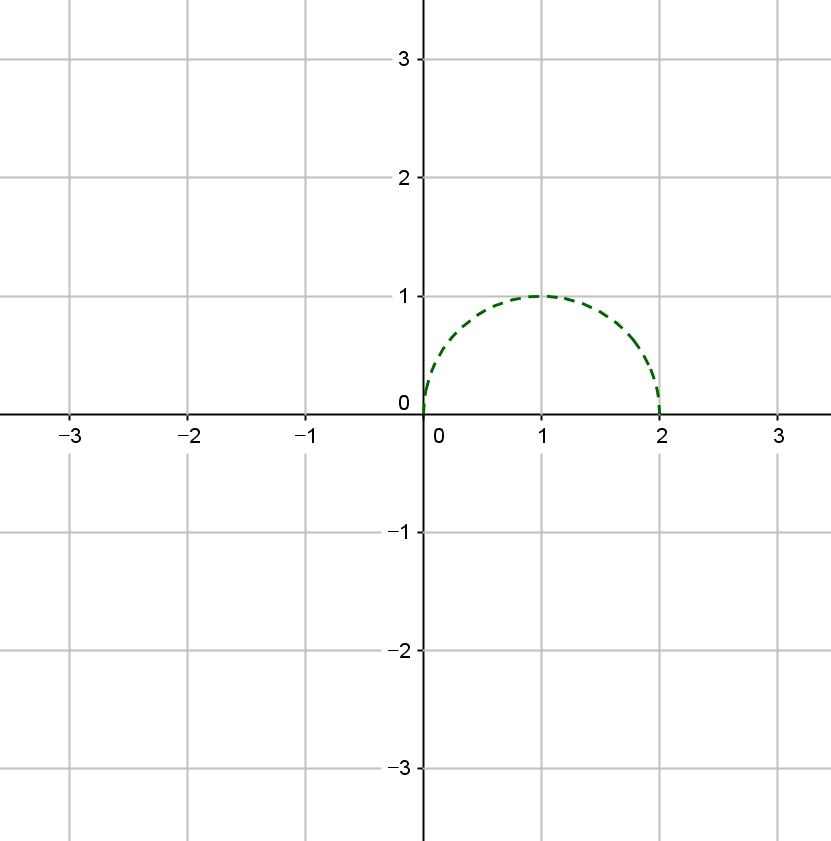
\includegraphics[width=0.49\textwidth]{review_2_2}}
&\raisebox{-.5\height}{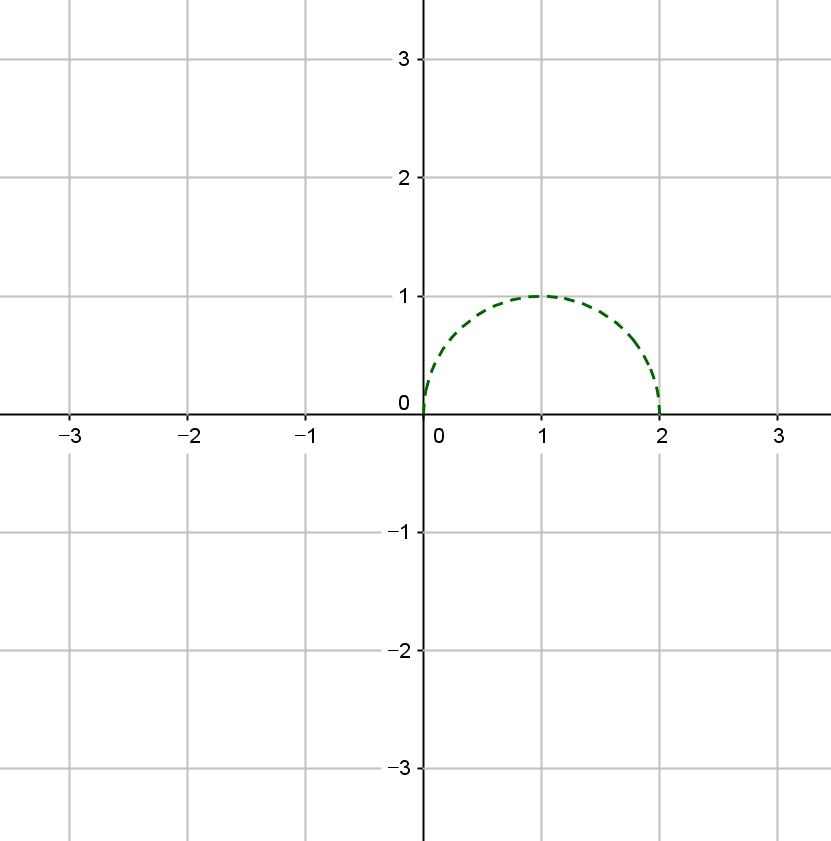
\includegraphics[width=0.49\textwidth]{review_2_2}}
\\\hline
\(y=f(x-1)\)&\(y=f(x)+2\)
\\
\(x\) 대신에 \pb{x+1}를 대입&\(y\) 대신에 \(y-2\)을 대입
\\
\(x\)축 방향으로 \(1\)만큼 평행이동&\(y\)축 방향으로 \pb{2}만큼 평행이동
\\\hline
\end{tabular}
}

\par\noindent
{\footnotesize
\begin{tabular}{p{0.49\textwidth}|p{0.49\textwidth}}
\hline
\raisebox{-.5\height}{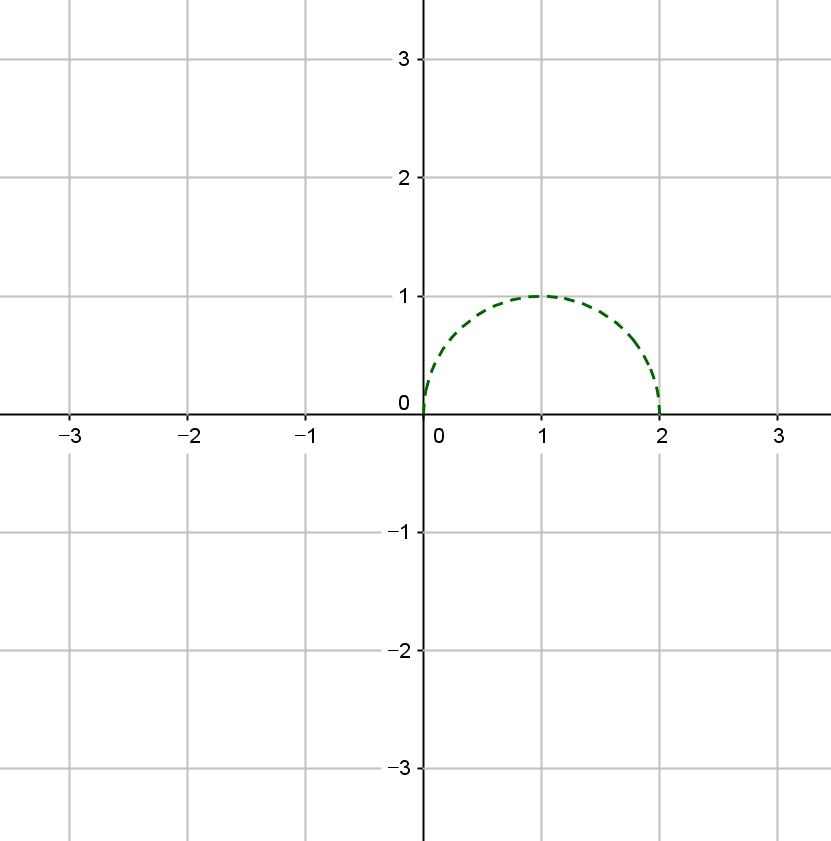
\includegraphics[width=0.49\textwidth]{review_2_2}}
&\raisebox{-.5\height}{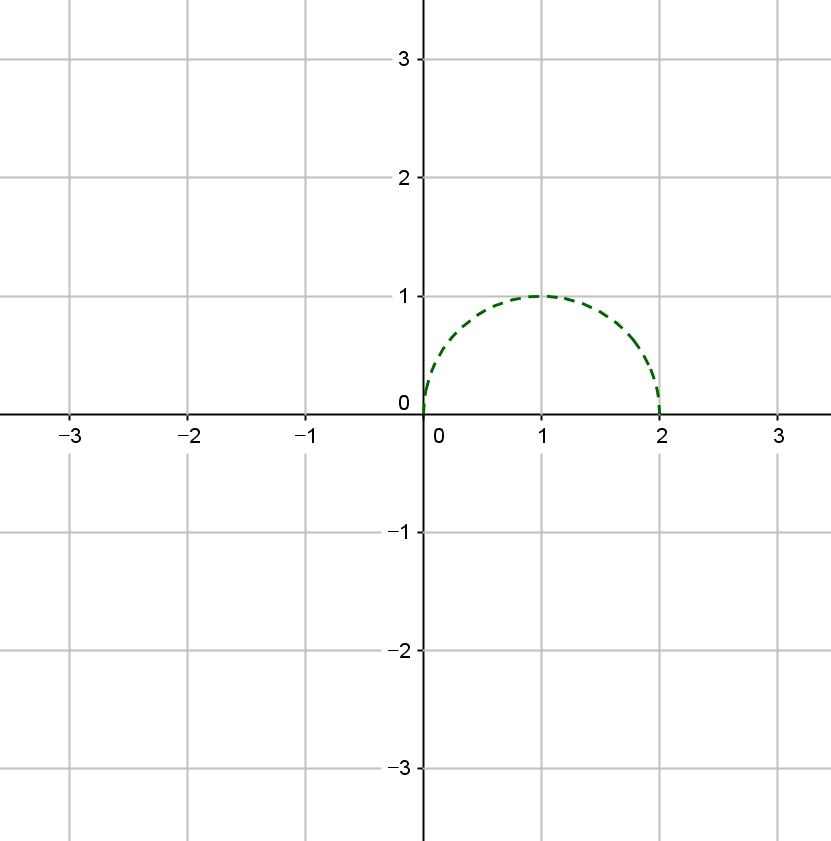
\includegraphics[width=0.49\textwidth]{review_2_2}}
\\\hline
\(y=f(x-1)+2\)&\(y=f(-x)\)
\\
\(x\), \(y\) 대신에 각각 \(x-1\),  \(y-2\)을 대입
& \(x\) 대신에 \pb{-x}를 대입
\\
\(x\)축, \(y\)축 방향으로 \(1\), \(2\)만큼 평행이동
&\(y\)축을 중심으로 대칭이동
\\\hline
\end{tabular}
}

\par\noindent
{\footnotesize
\begin{tabular}{p{0.49\textwidth}|p{0.49\textwidth}}
\raisebox{-.5\height}{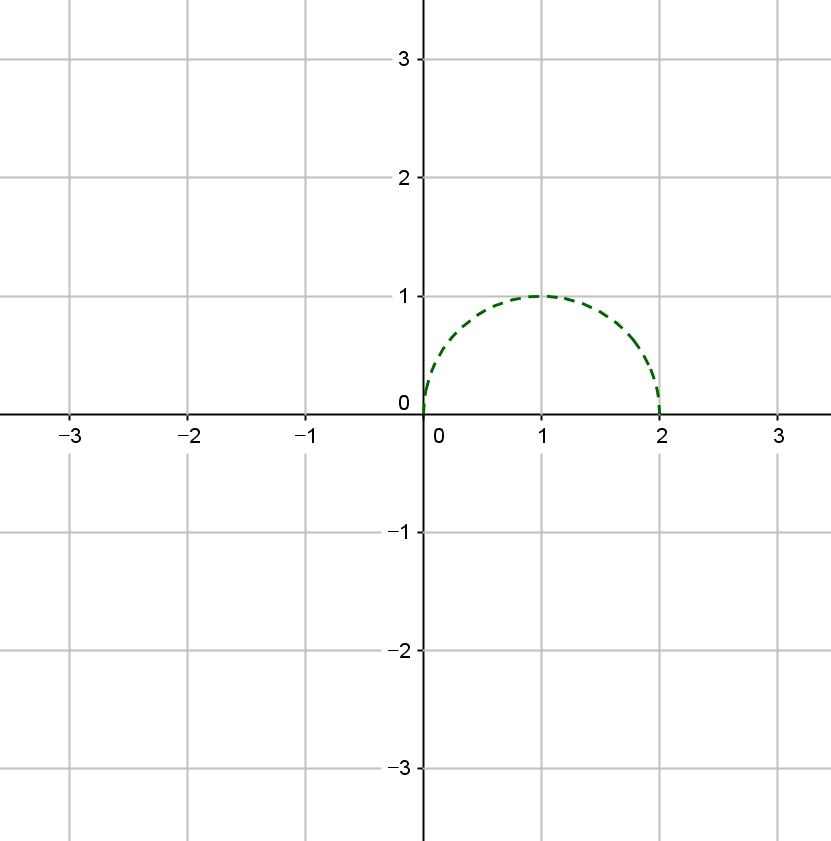
\includegraphics[width=0.49\textwidth]{review_2_2}}
&\raisebox{-.5\height}{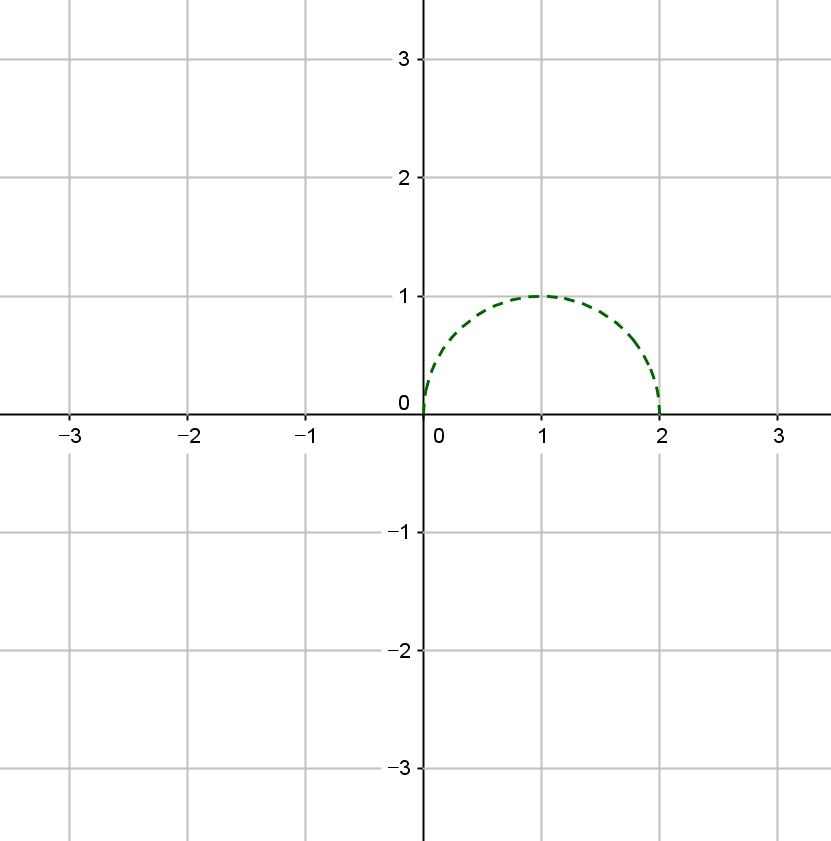
\includegraphics[width=0.49\textwidth]{review_2_2}}
\\\hline
\(y=-f(x)\)&\(y=-f(-x)\)
\\
\(y\) 대신에 \(-y\)를 대입
& \(x\), \(y\) 대신에 각각 \(-x\), \(-y\)를 대입
\\
\pb{x축}을 중심으로 대칭이동
&\pb{원점}을 중심으로 대칭이동
\\\hline
\end{tabular}
}

%%%
%\subsection{\(y=2f(x)\)의 그래프 그리기}
%\(y=f(x)\)의 그래프는 \((1,f(1))\), \((2,f(2))\), \((3,f(3))\) 등의 점을 지난다.
%반면 \(y=2f(x)\)의 그래프는 \((1,2f(1))\), \((2,2f(2))\), \((3,2f(3))\) 등의 점을 지나야 한다.
%따라서 주어진 \(y=f(x)\) 그래프를 세로방향으로 두 배 늘리면 \(y=2f(x)\)의 그래프가 된다.
%
%%
%\prob{}
%다음 그래프들을 그리시오.
%
%\par\noindent
%{\footnotesize
%\begin{tabular}{c|c}
%\hline
%\raisebox{-.5\height}{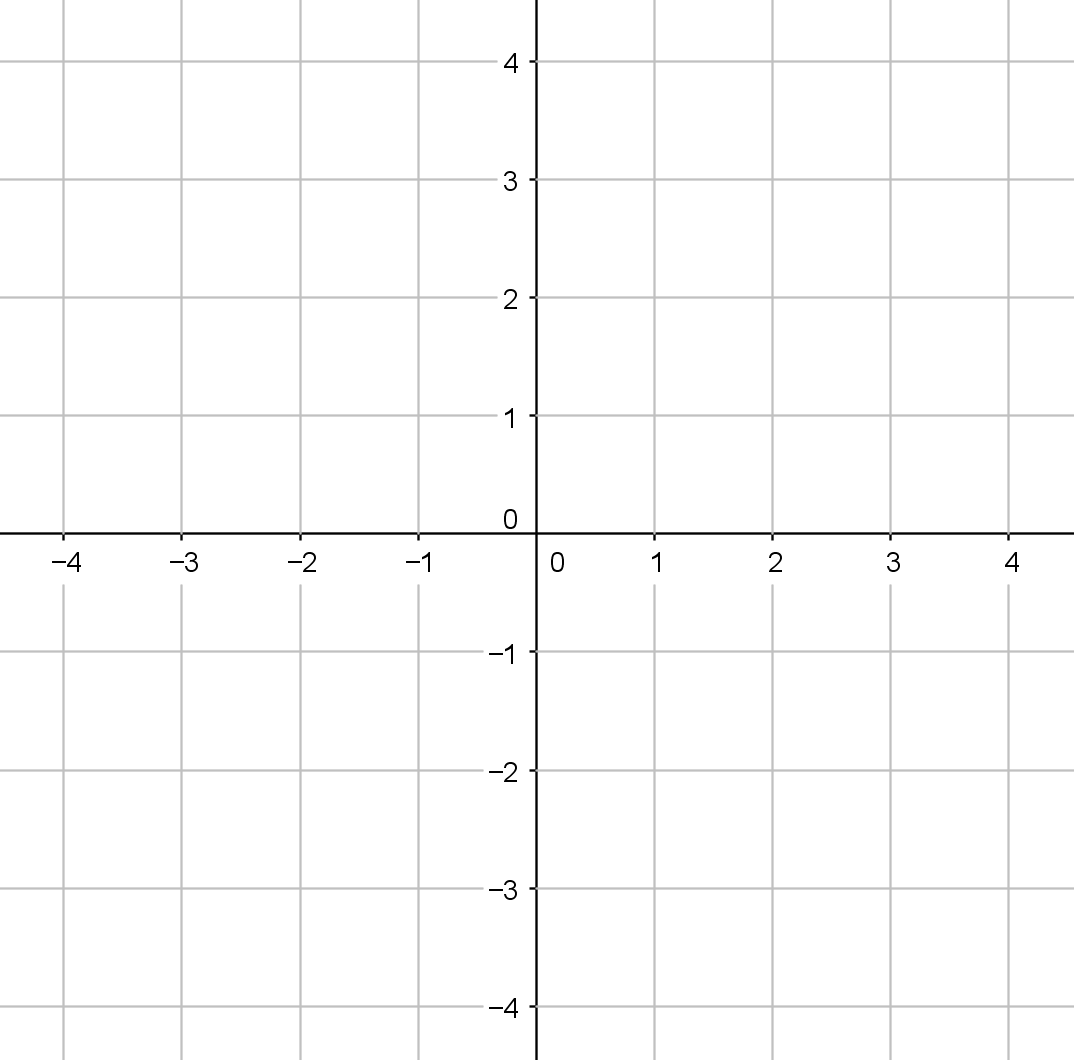
\includegraphics[width=0.49\textwidth]{grid_4}}
%&\raisebox{-.5\height}{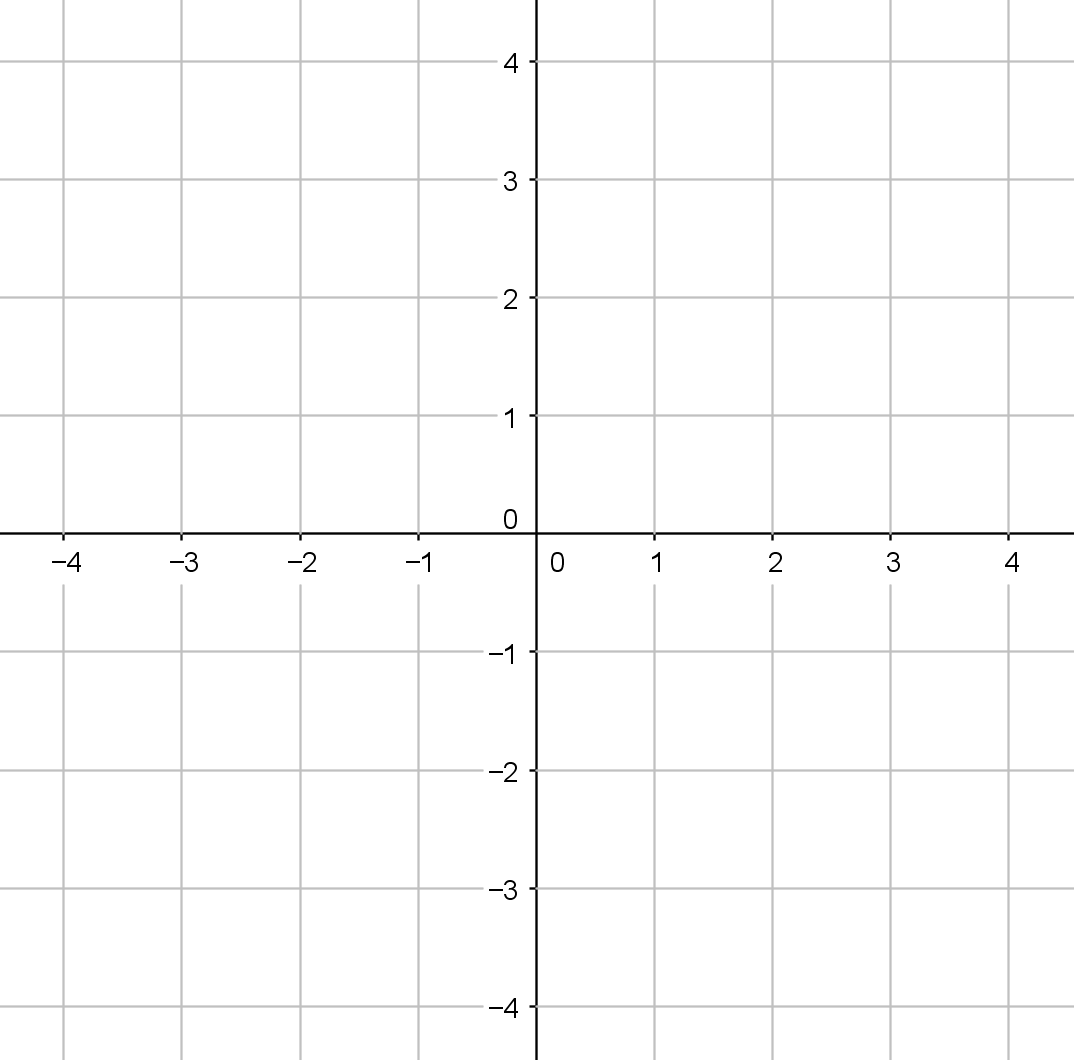
\includegraphics[width=0.49\textwidth]{grid_4}}
%\\\hline
%\(y=2x\)&\(y=4x\)
%\\\hline
%\end{tabular}
%}
%
%\par\noindent
%{\footnotesize
%\begin{tabular}{c|c}
%\hline
%\raisebox{-.5\height}{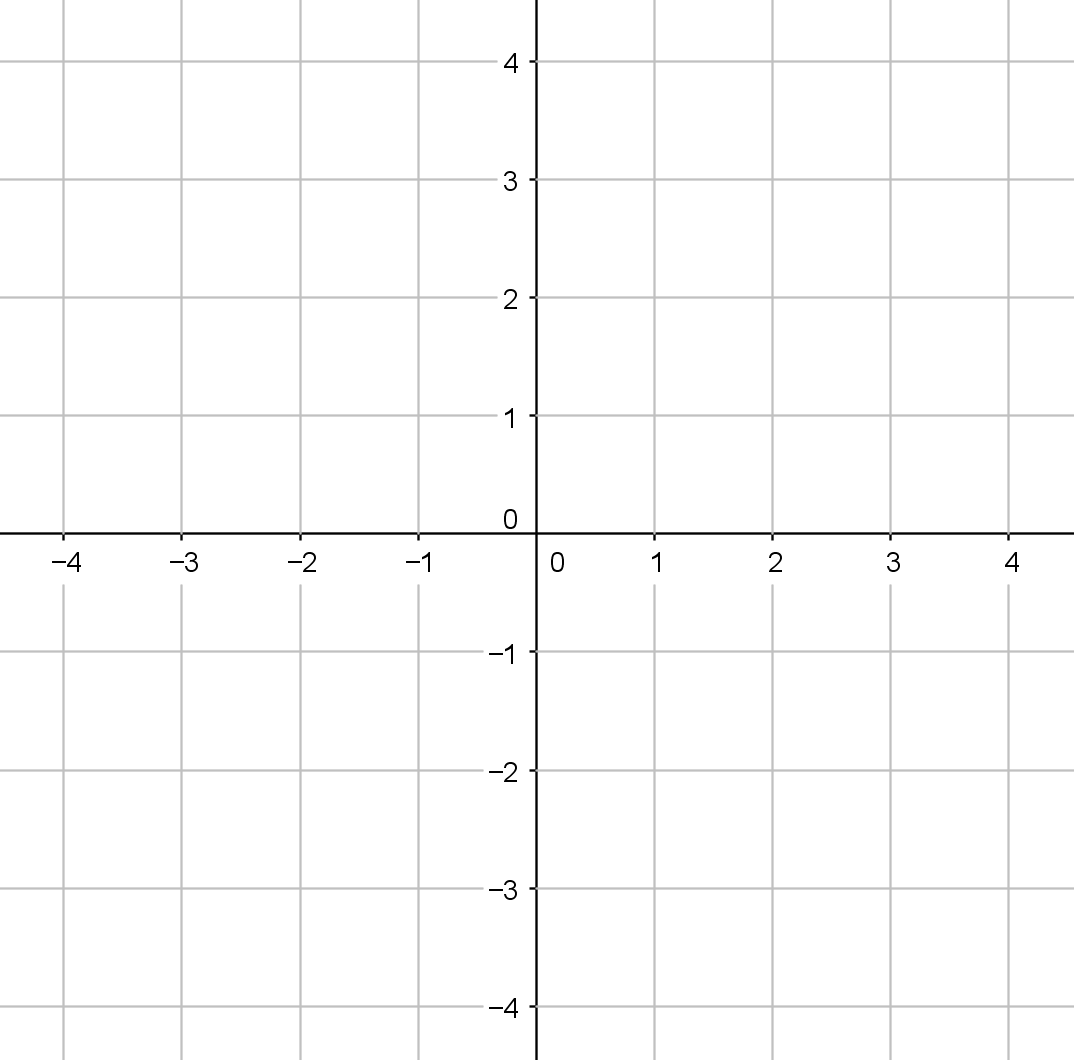
\includegraphics[width=0.49\textwidth]{grid_4}}
%&\raisebox{-.5\height}{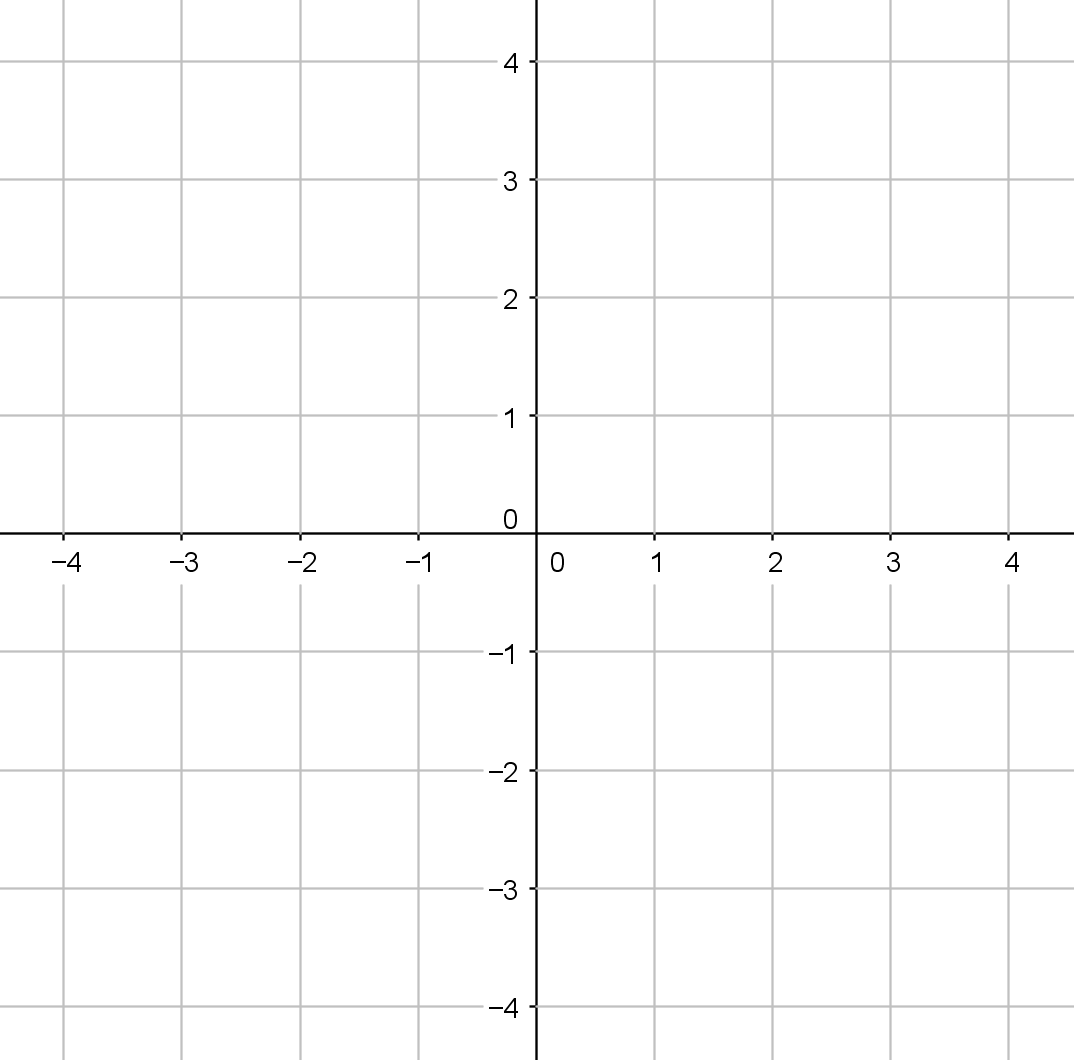
\includegraphics[width=0.49\textwidth]{grid_4}}
%\\\hline
%\(y=\frac13x+1\)&\(y=\frac23x+2\)
%\\\hline
%\end{tabular}
%}
%
%\par\noindent
%{\footnotesize
%\begin{tabular}{c|c}
%\hline
%\raisebox{-.5\height}{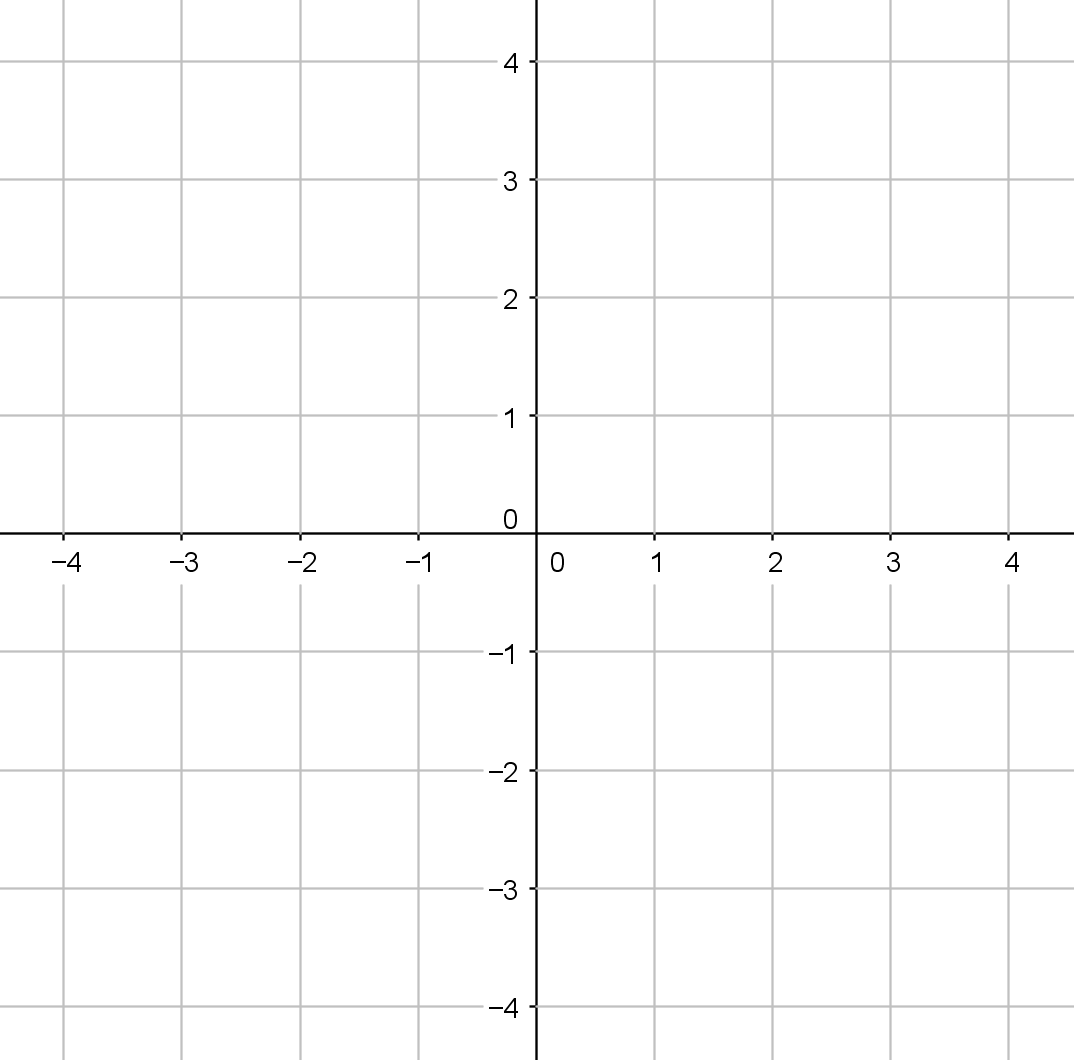
\includegraphics[width=0.49\textwidth]{grid_4}}
%&\raisebox{-.5\height}{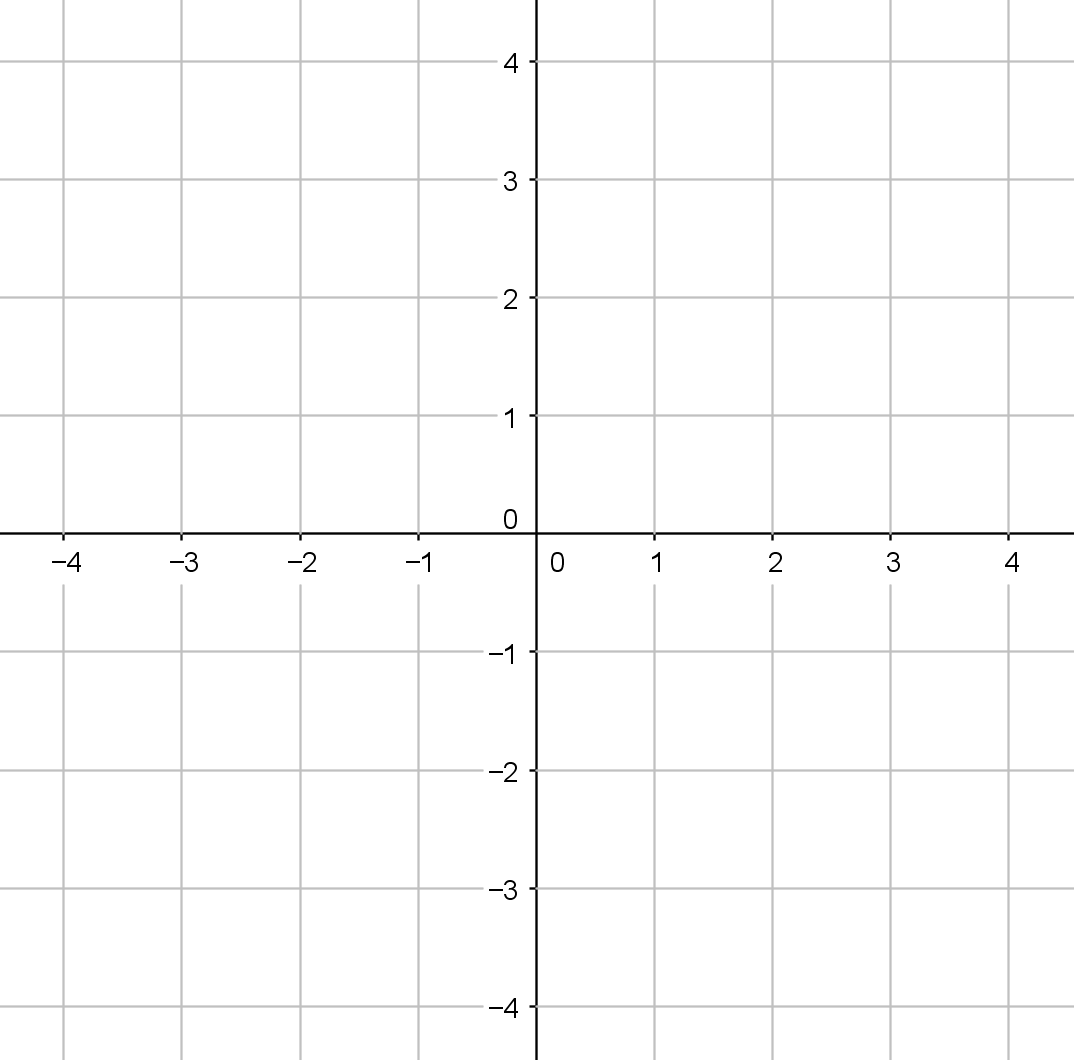
\includegraphics[width=0.49\textwidth]{grid_4}}
%\\\hline
%\(y=x^2\)&\(y=2x^2\)
%\\\hline
%\end{tabular}
%}
%
%\par\noindent
%{\footnotesize
%\begin{tabular}{c|c}
%\hline
%\raisebox{-.5\height}{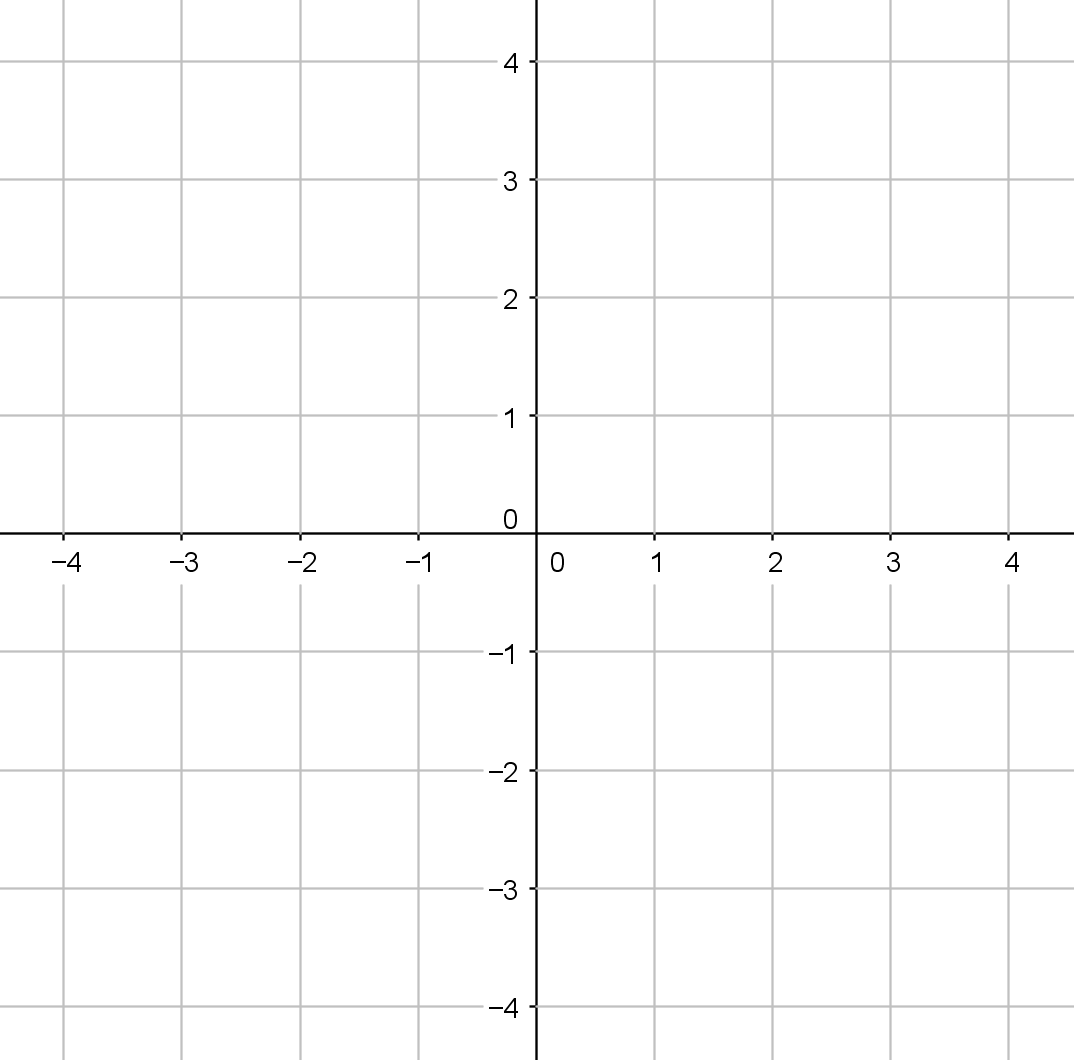
\includegraphics[width=0.49\textwidth]{grid_4}}
%&\raisebox{-.5\height}{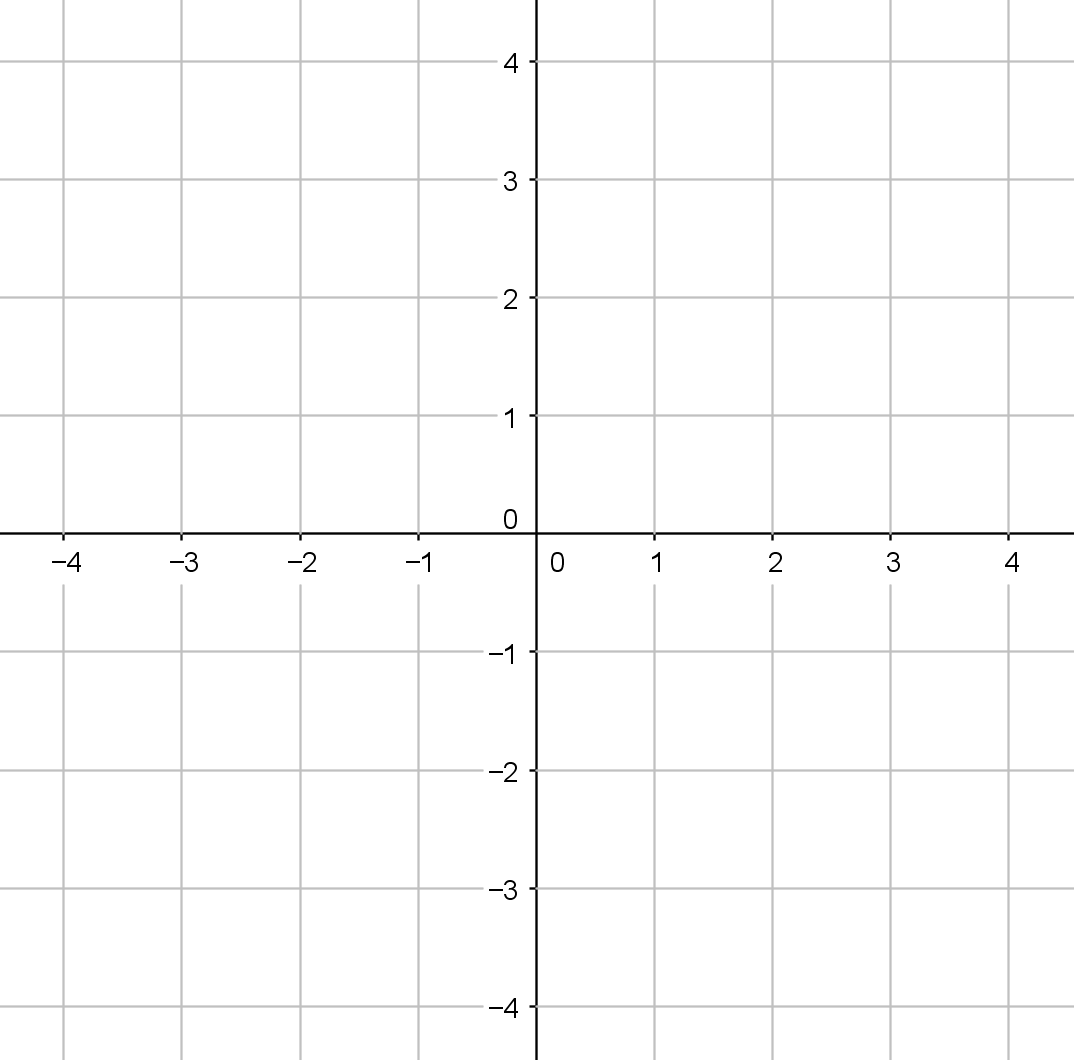
\includegraphics[width=0.49\textwidth]{grid_4}}
%\\\hline
%\(y=x^2-2x\)&\(y=2x^2-4x\)
%\\\hline
%\end{tabular}
%}
%
%\par\noindent
%{\footnotesize
%\begin{tabular}{c|c}
%\hline
%\raisebox{-.5\height}{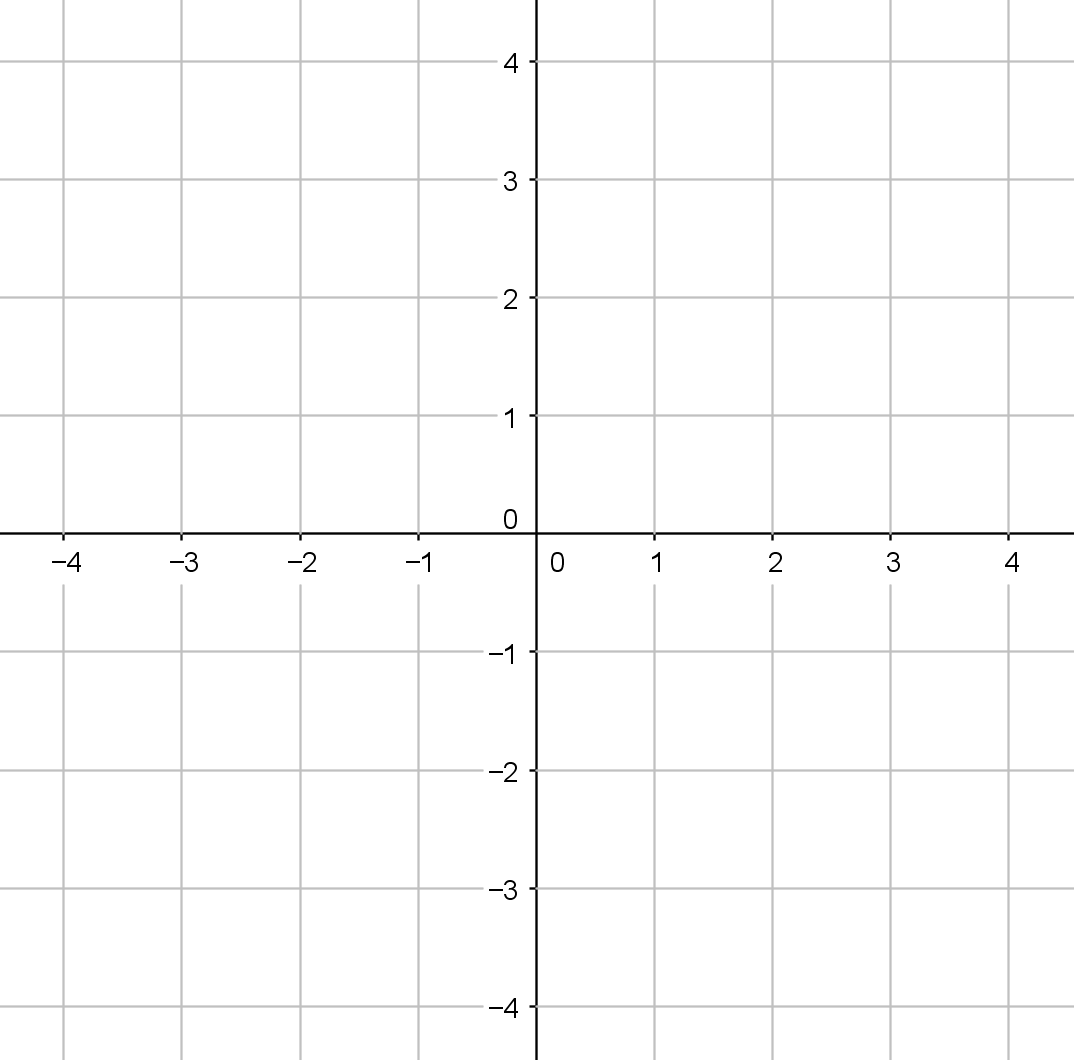
\includegraphics[width=0.49\textwidth]{grid_4}}
%&\raisebox{-.5\height}{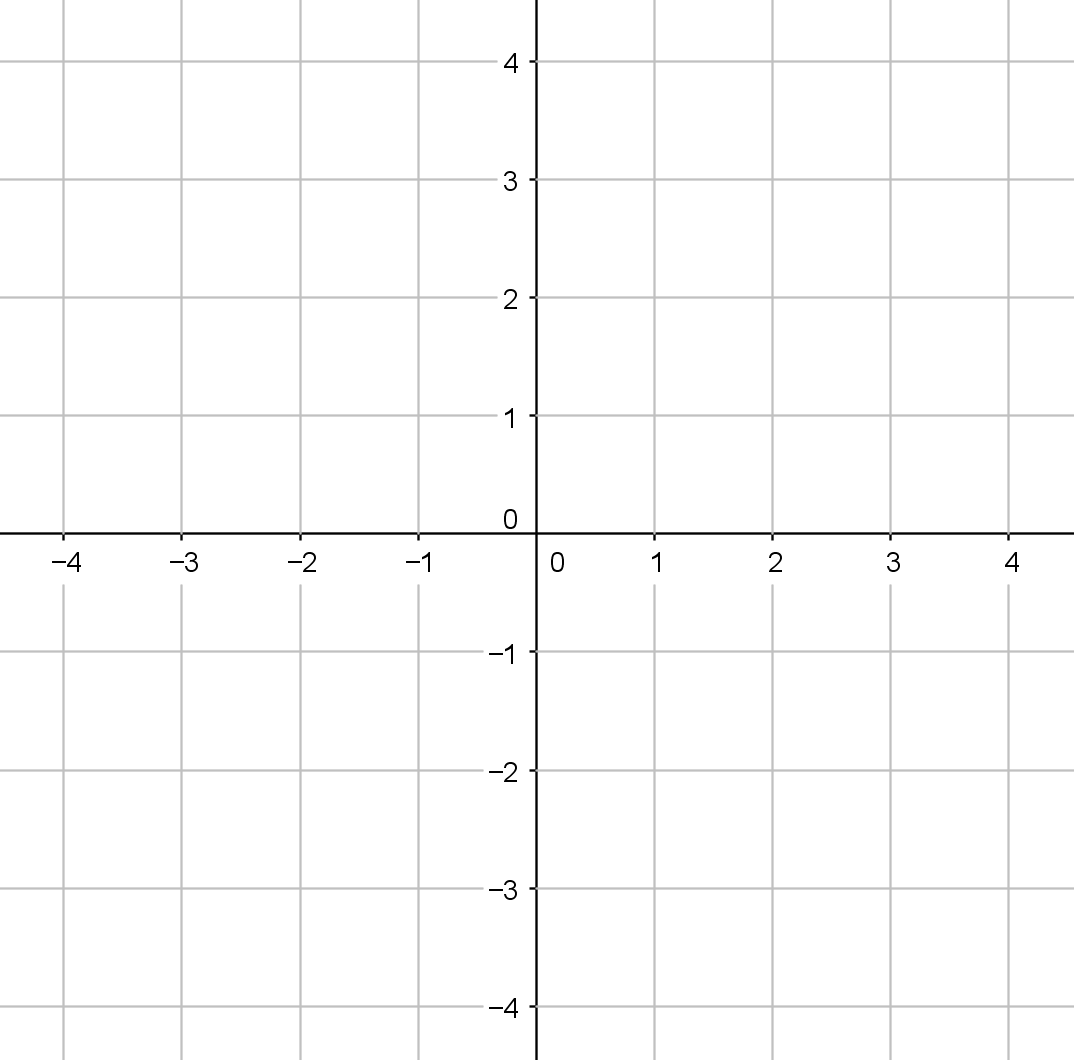
\includegraphics[width=0.49\textwidth]{grid_4}}
%\\\hline
%\(y=\frac2x\)&\(y=\frac4x\)
%\\\hline
%\end{tabular}
%}
%
%\par\noindent
%{\footnotesize
%\begin{tabular}{c|c}
%\hline
%\raisebox{-.5\height}{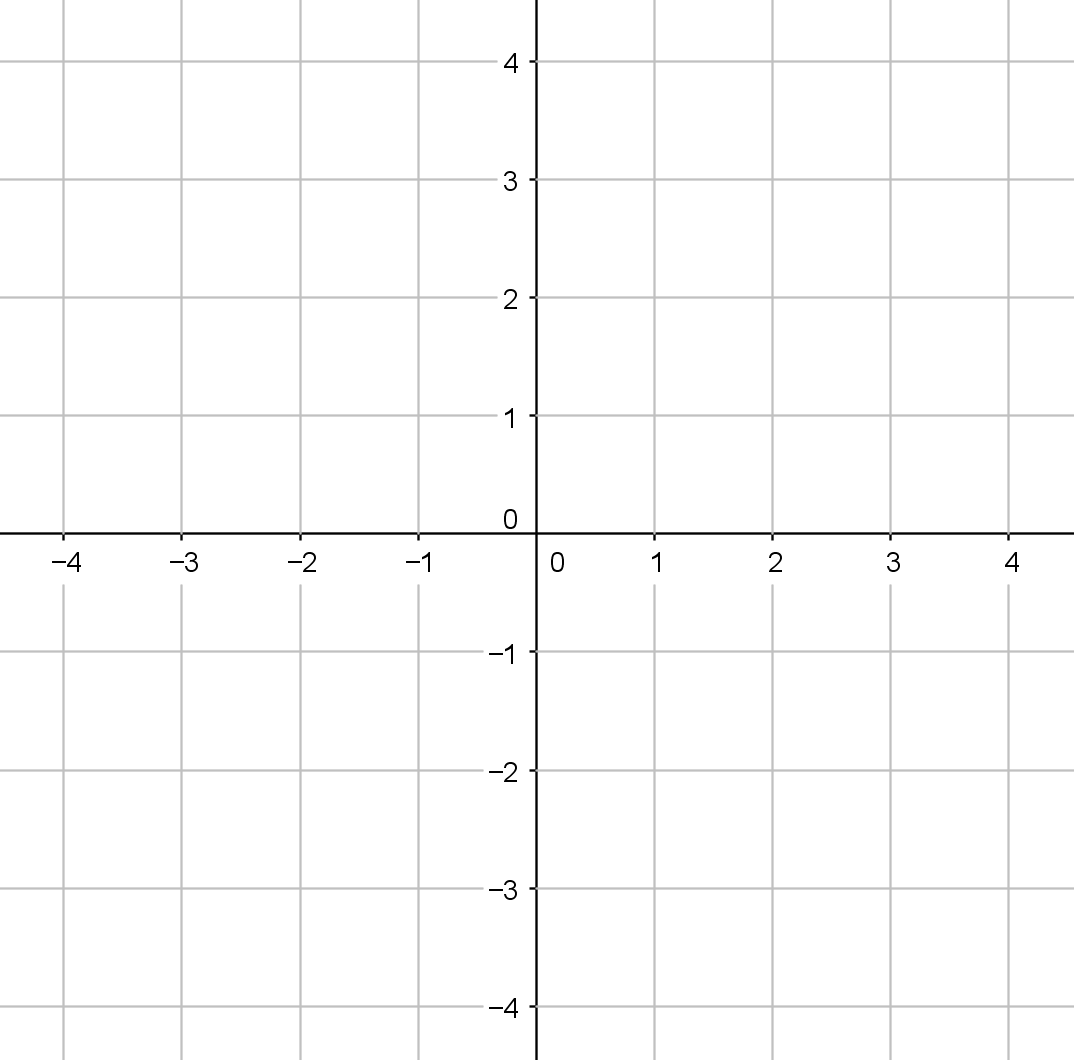
\includegraphics[width=0.49\textwidth]{grid_4}}
%&\raisebox{-.5\height}{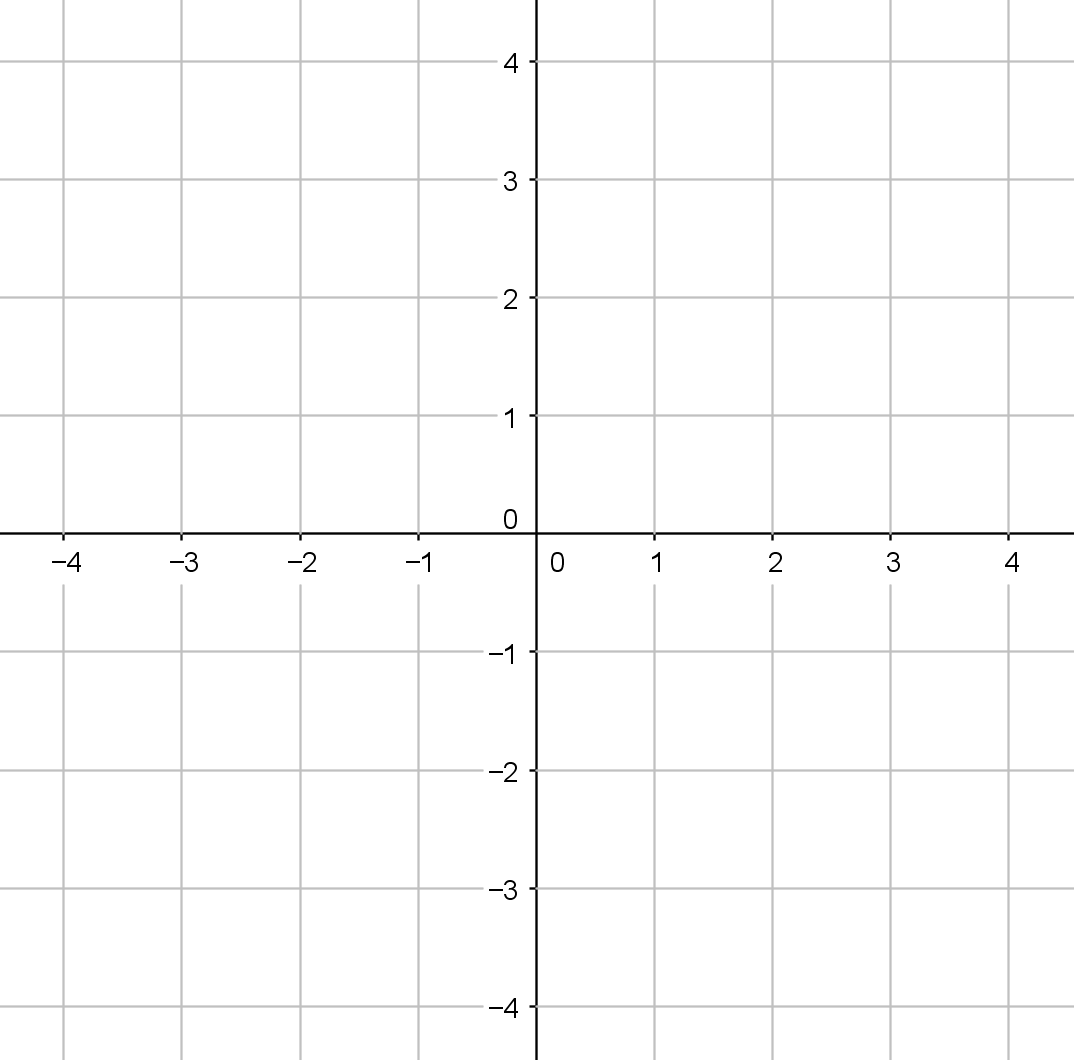
\includegraphics[width=0.49\textwidth]{grid_4}}
%\\\hline
%\(y=\frac{2x-1}{x-1}\)&\(y=\frac{4x-2}{x-1}\)
%\\\hline
%\end{tabular}
%}
%
%%%
%\subsection{\(y=\frac12f(x)\)의 그래프 그리기}
%\(y=\frac12f(x)\)의 그래프는 \((1,\frac12f(1))\), \((2,\frac12f(2))\), \((3,\frac12f(3))\) 등의 점을 지나야 한다.
%따라서 주어진 \(y=f(x)\) 그래프를 세로방향으로 두 배 축소시키면면 \(y=\frac12f(x)\)의 그래프가 된다.
%
%%
%\prob{}
%다음 그래프들을 그리시오.
%
%\par\noindent
%{\footnotesize
%\begin{tabular}{c|c}
%\hline
%\raisebox{-.5\height}{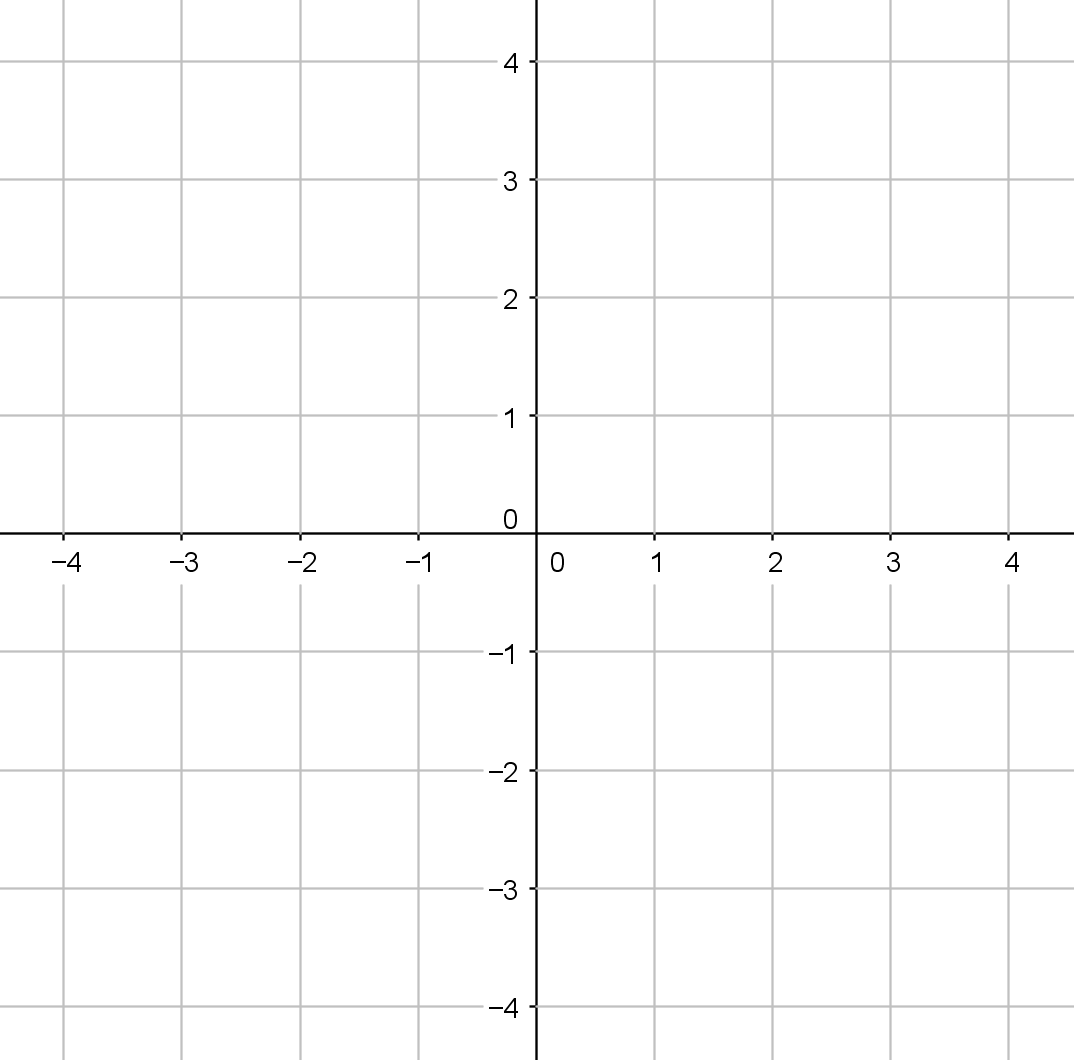
\includegraphics[width=0.49\textwidth]{grid_4}}
%&\raisebox{-.5\height}{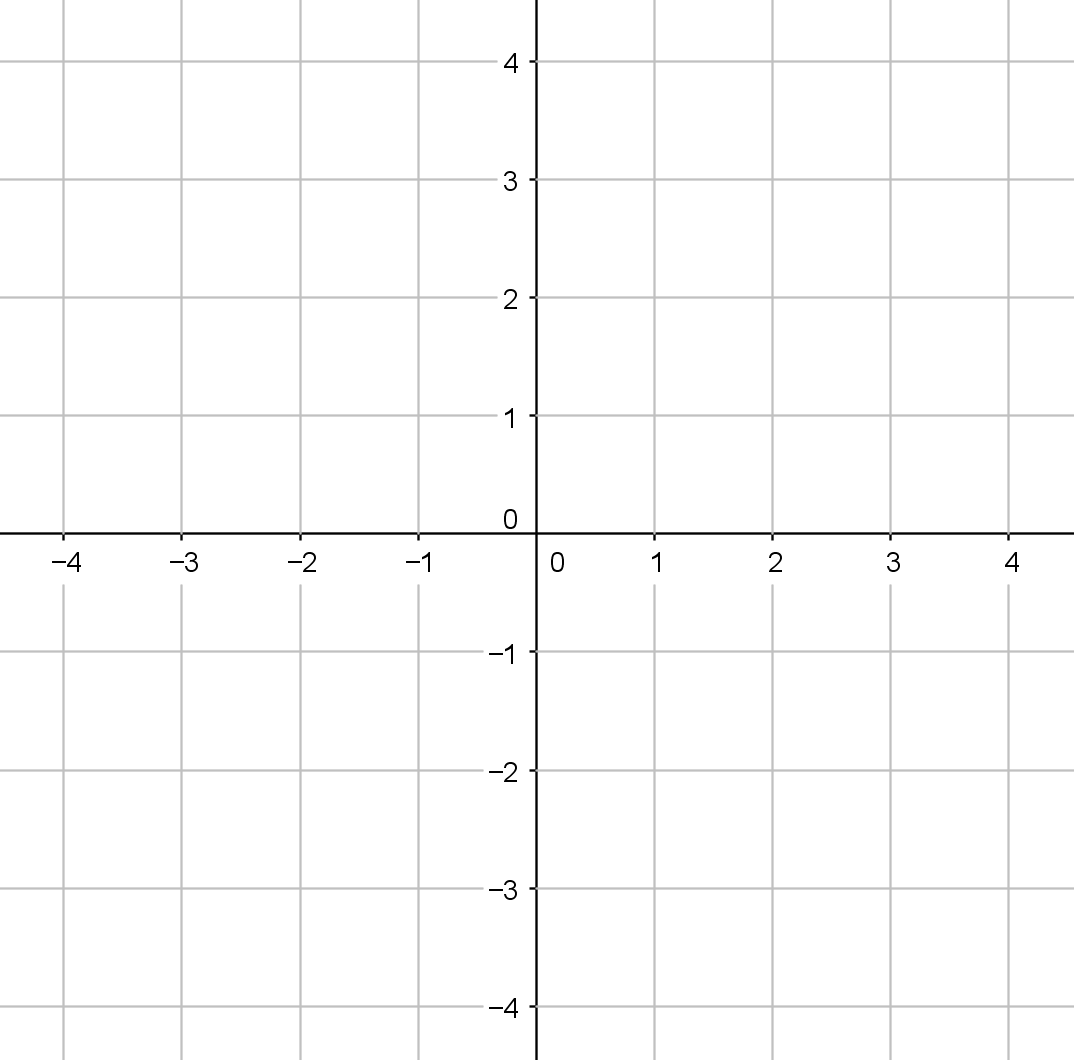
\includegraphics[width=0.49\textwidth]{grid_4}}
%\\\hline
%\(y=2x\)&\(y=x\)
%\\\hline
%\end{tabular}
%}
%
%\par\noindent
%{\footnotesize
%\begin{tabular}{c|c}
%\hline
%\raisebox{-.5\height}{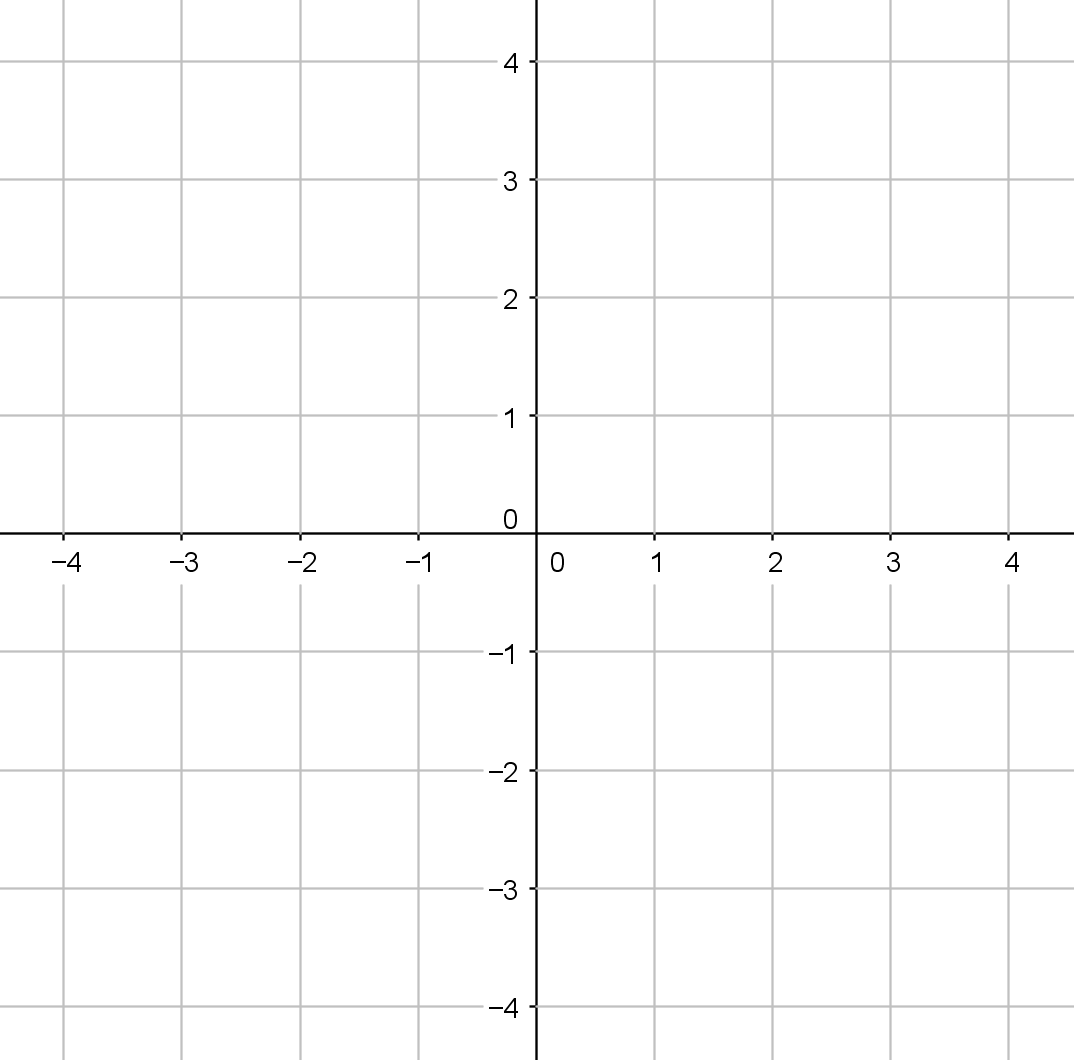
\includegraphics[width=0.49\textwidth]{grid_4}}
%&\raisebox{-.5\height}{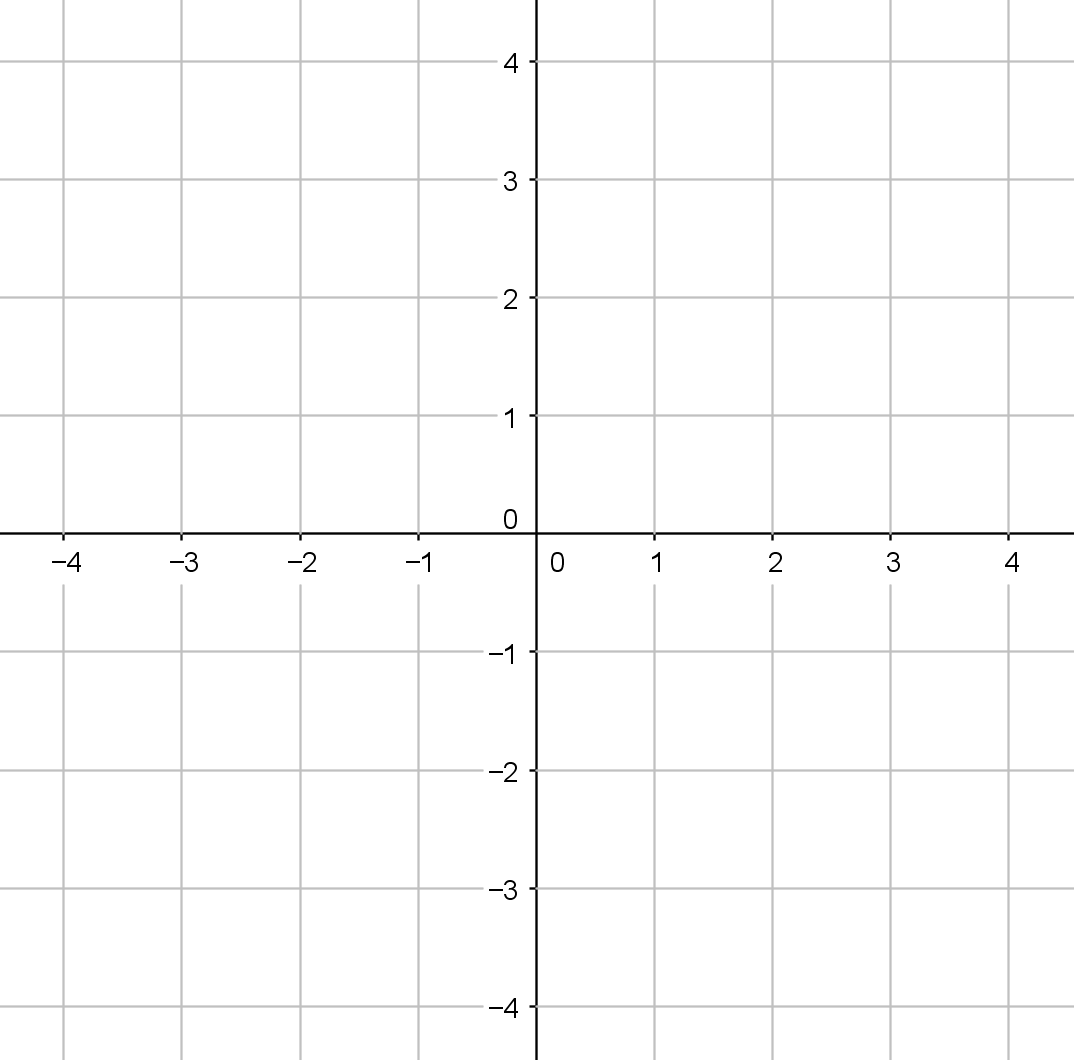
\includegraphics[width=0.49\textwidth]{grid_4}}
%\\\hline
%\(y=\frac13x+1\)&\(y=\frac16x+\frac12\)
%\\\hline
%\end{tabular}
%}
%
%\par\noindent
%{\footnotesize
%\begin{tabular}{c|c}
%\hline
%\raisebox{-.5\height}{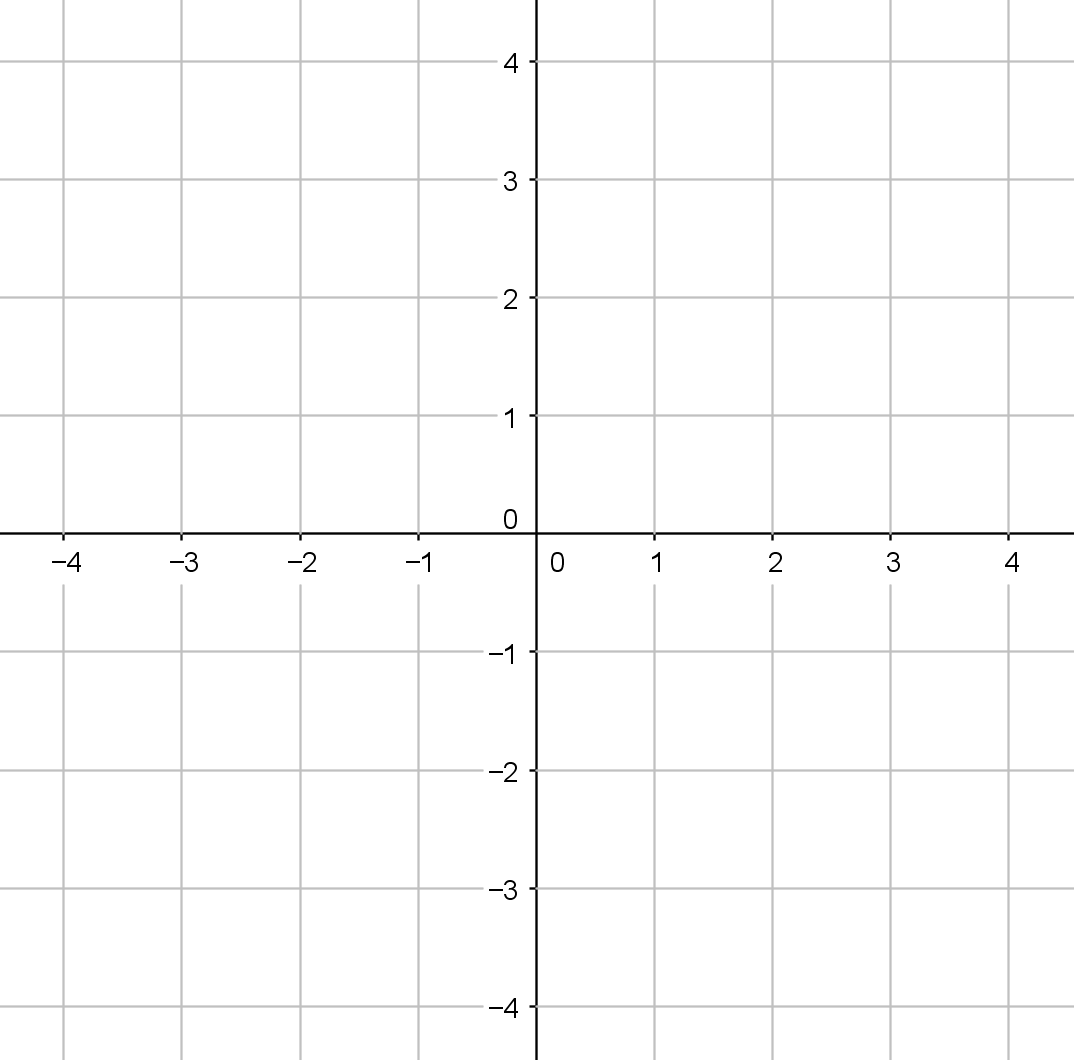
\includegraphics[width=0.49\textwidth]{grid_4}}
%&\raisebox{-.5\height}{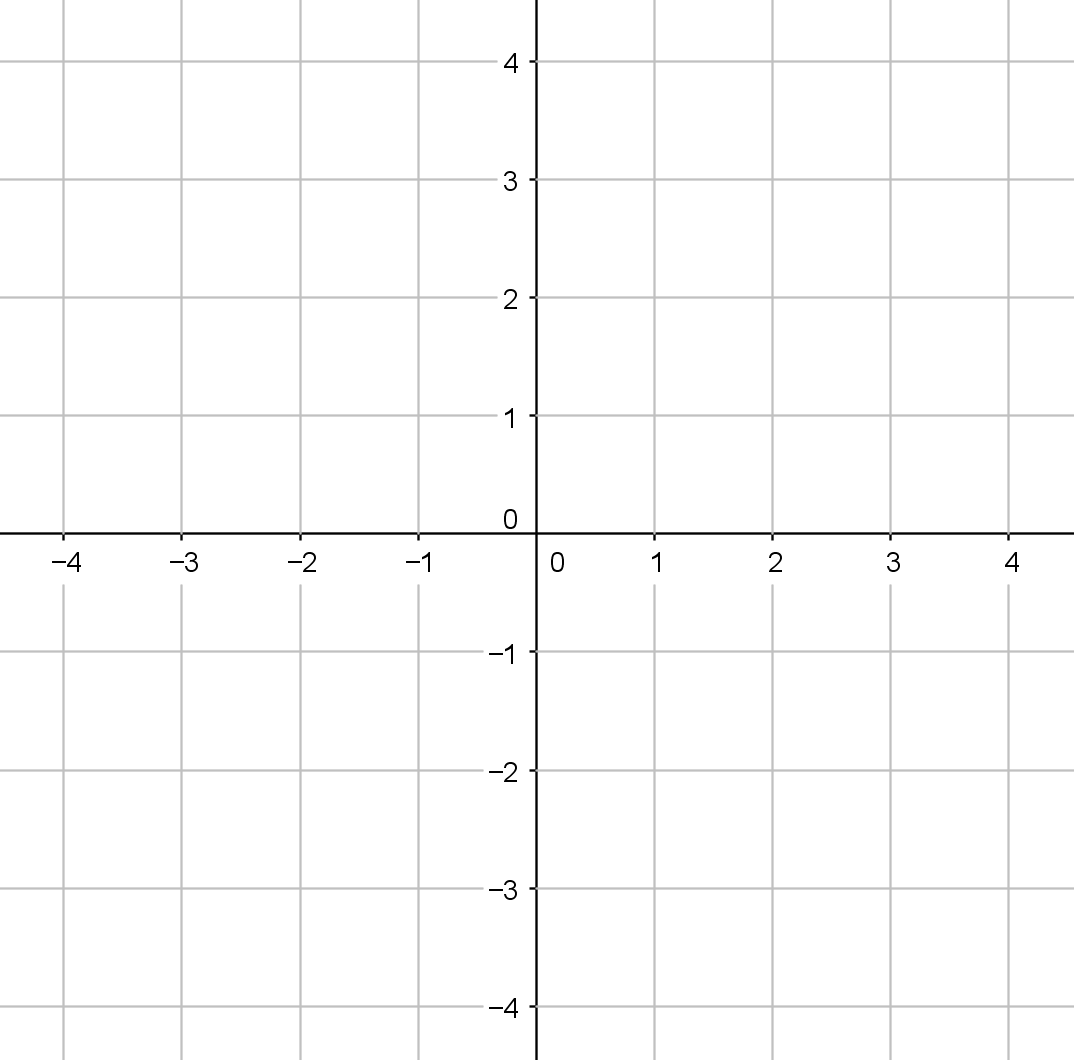
\includegraphics[width=0.49\textwidth]{grid_4}}
%\\\hline
%\(y=x^2\)&\(y=\frac12x^2\)
%\\\hline
%\end{tabular}
%}
%
%\par\noindent
%{\footnotesize
%\begin{tabular}{c|c}
%\hline
%\raisebox{-.5\height}{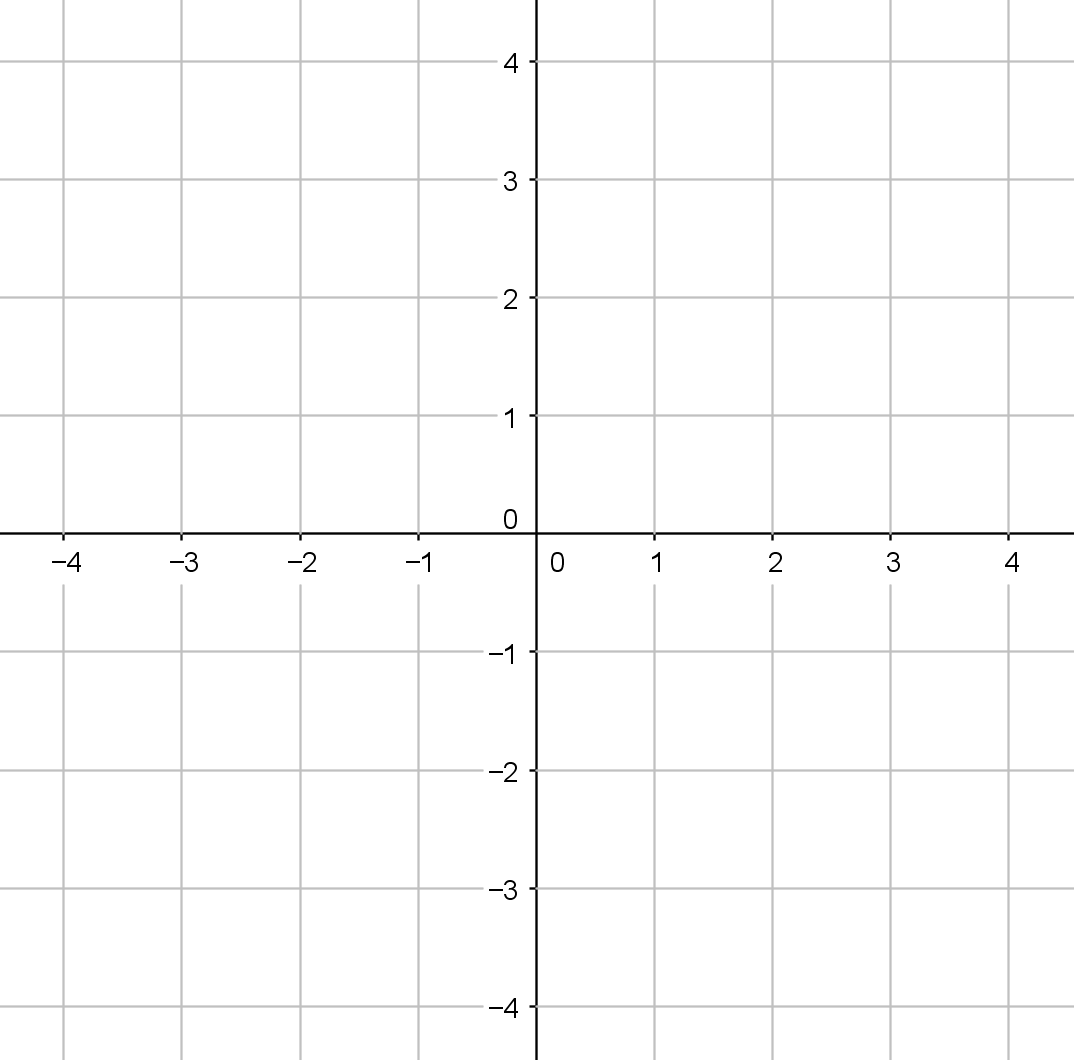
\includegraphics[width=0.49\textwidth]{grid_4}}
%&\raisebox{-.5\height}{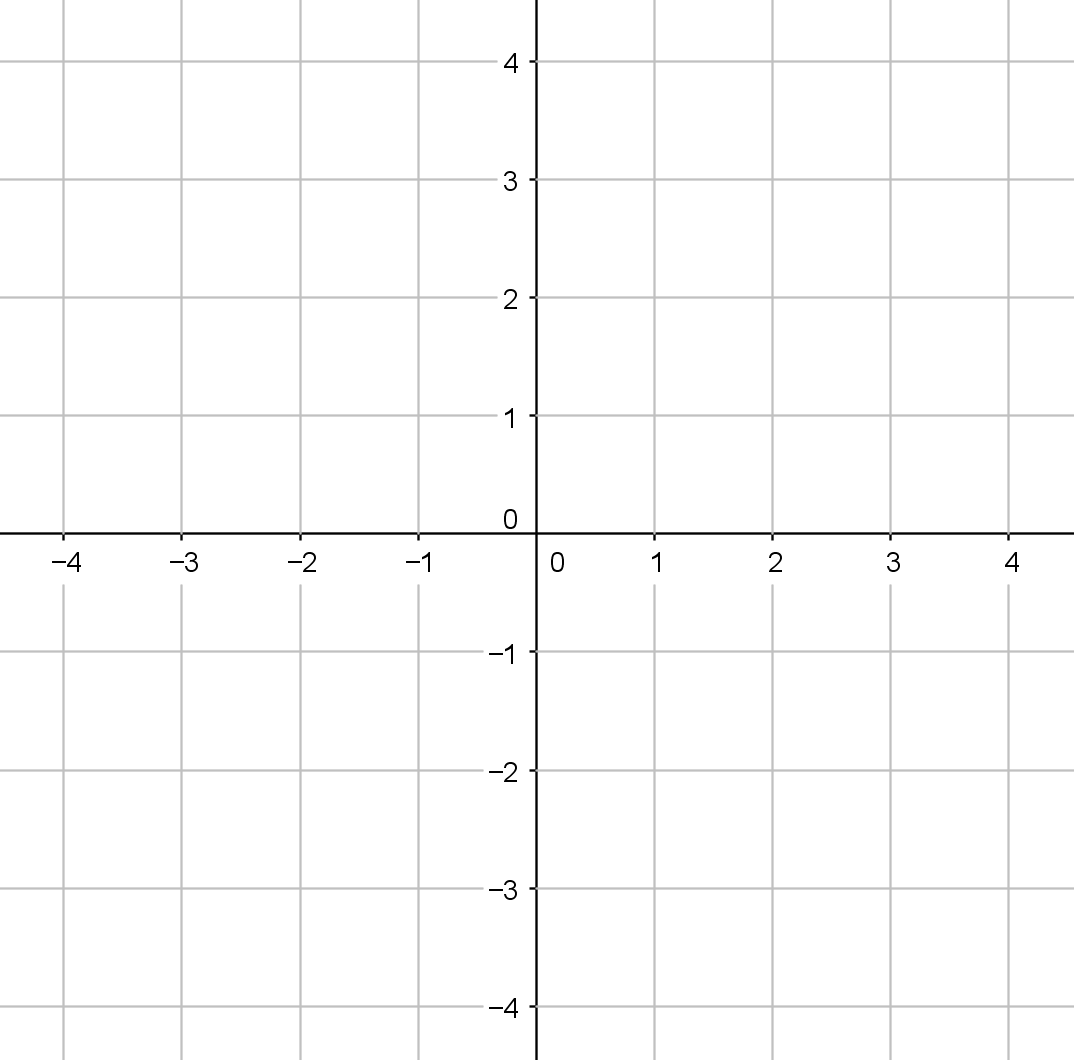
\includegraphics[width=0.49\textwidth]{grid_4}}
%\\\hline
%\(y=x^2-2x\)&\(y=\frac12x^2-x\)
%\\\hline
%\end{tabular}
%}
%
%\par\noindent
%{\footnotesize
%\begin{tabular}{c|c}
%\hline
%\raisebox{-.5\height}{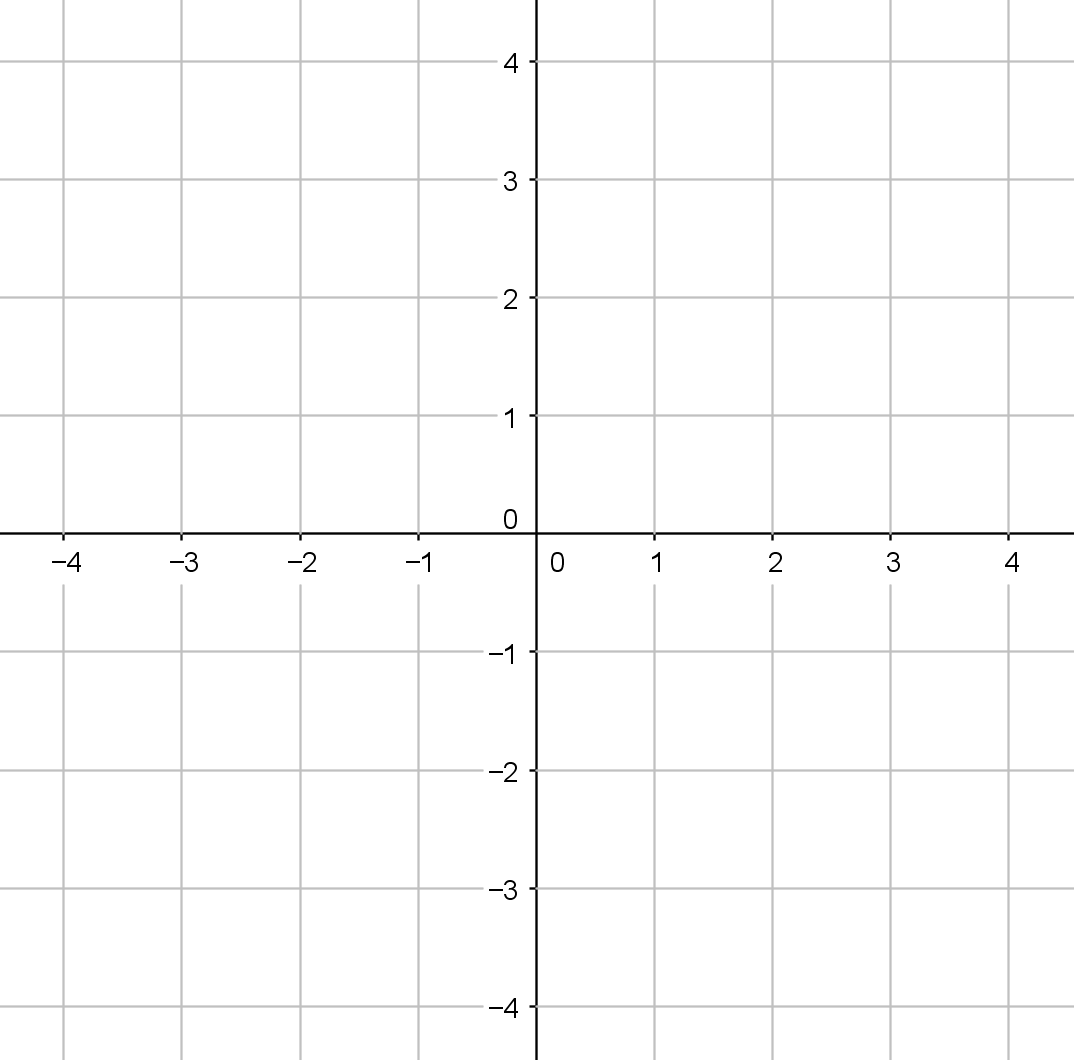
\includegraphics[width=0.49\textwidth]{grid_4}}
%&\raisebox{-.5\height}{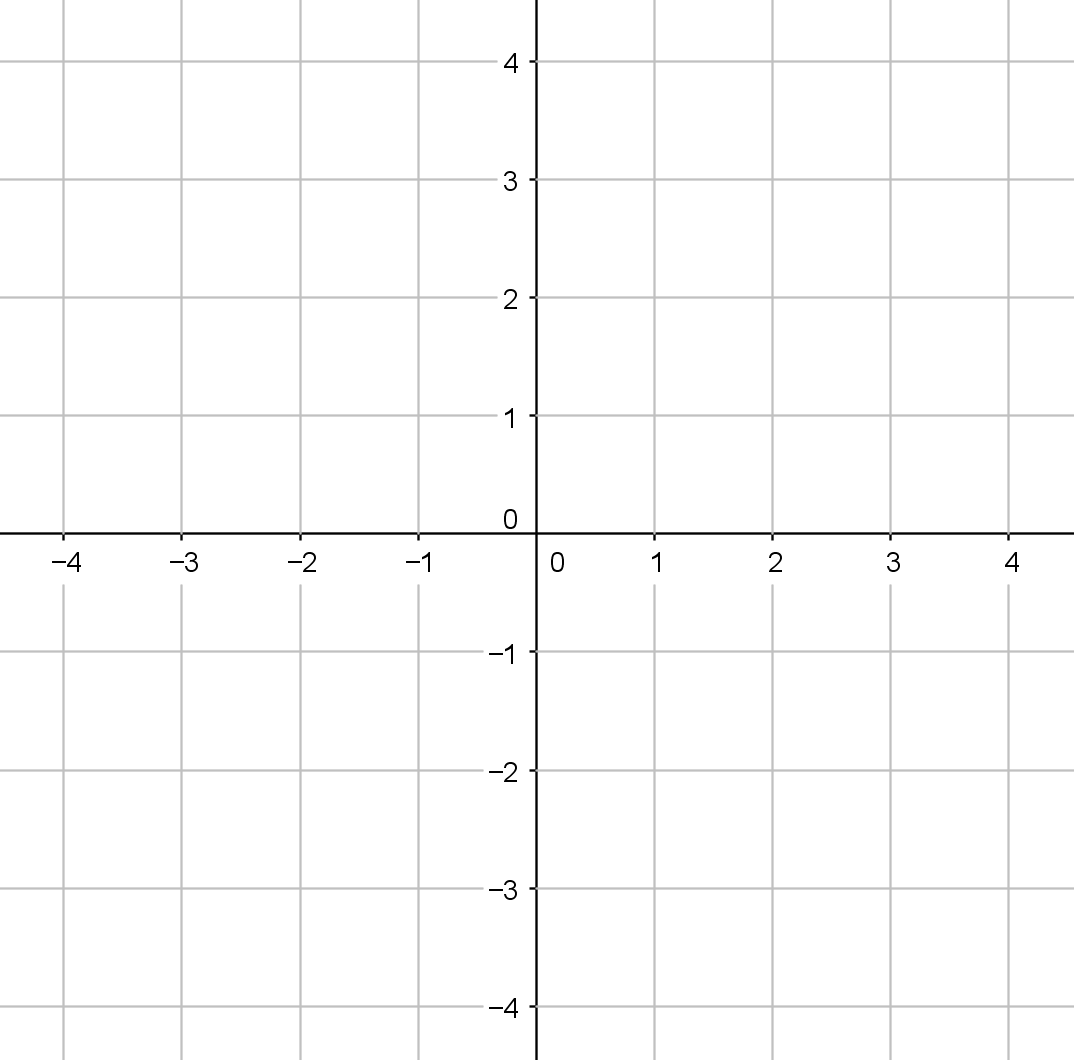
\includegraphics[width=0.49\textwidth]{grid_4}}
%\\\hline
%\(y=\frac2x\)&\(y=\frac1x\)
%\\\hline
%\end{tabular}
%}
%
%\par\noindent
%{\footnotesize
%\begin{tabular}{c|c}
%\hline
%\raisebox{-.5\height}{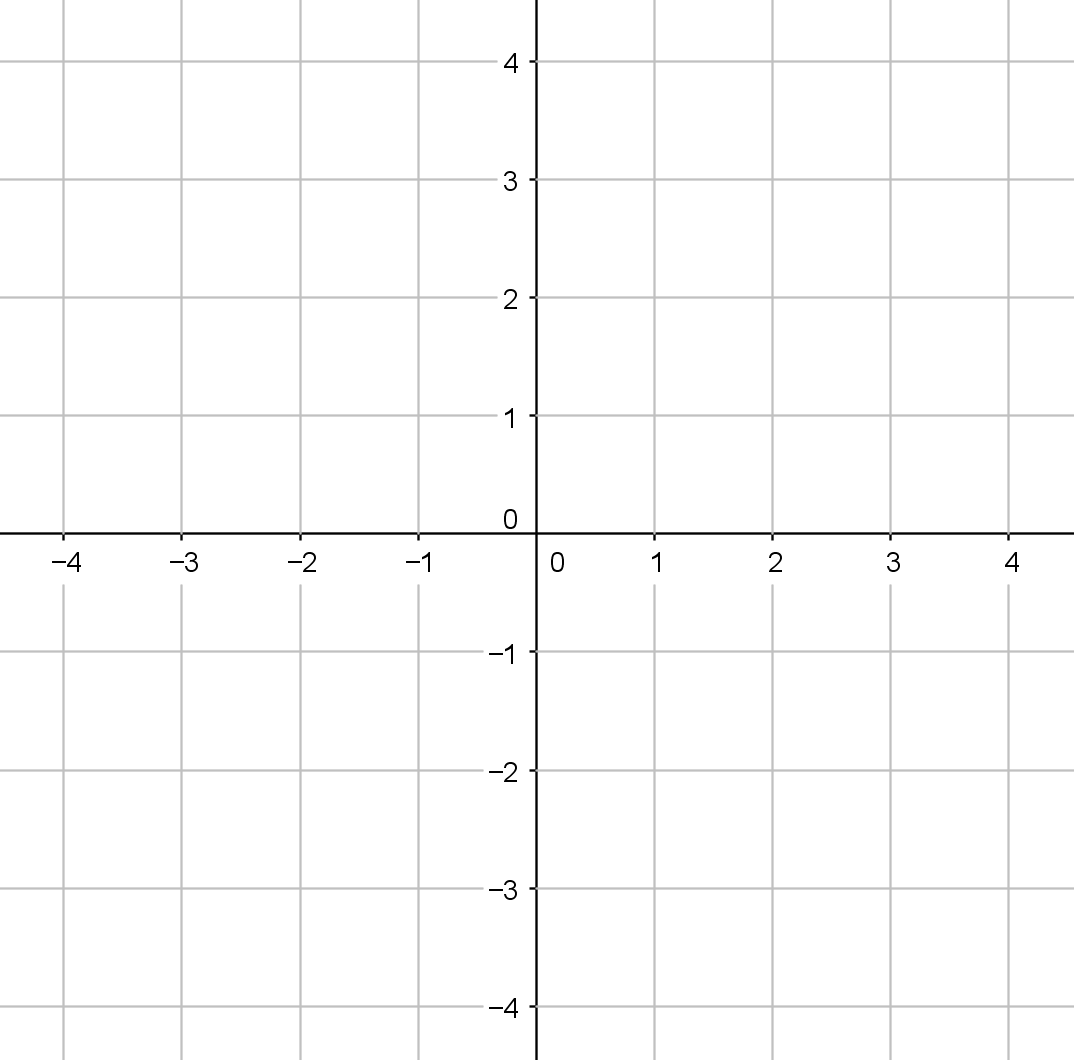
\includegraphics[width=0.49\textwidth]{grid_4}}
%&\raisebox{-.5\height}{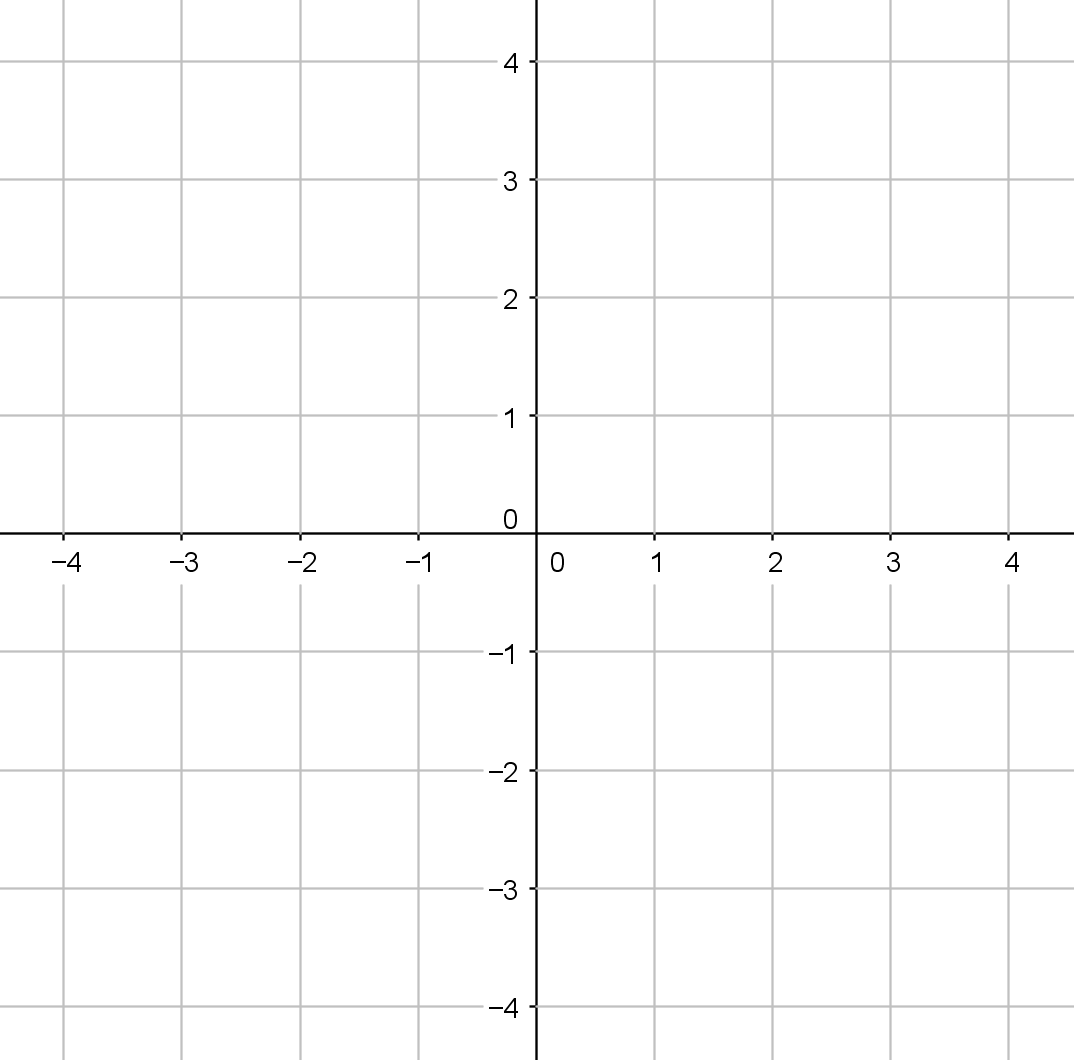
\includegraphics[width=0.49\textwidth]{grid_4}}
%\\\hline
%\(y=\frac{2x-1}{x-1}\)&\(y=\frac{x-\frac12}{x-1}\)
%\\\hline
%\end{tabular}
%}
%
%%%
%\subsection{\(y=kf(x)\)의 그래프 그리기}
%
%%
%\theo{}
%\(k>0\)일 때,
%\(y=kf(x)\)의 그래프는,
%\begin{enumerate}[i)]
%\item
%(\(k>1\)일 때) \(y=f(x)\)의 그래프를 세로로 \(k\)배 만큼 늘려서 얻을 수 있다.
%\item
%(\(0<k<1\)일 때) \(y=f(x)\)의 그래프를 세로로 \(k\)배 만큼 축소시켜서 얻을 수 있다.
%\end{enumerate}
%

\clearpage
%%%
\section{무리함수의 그래프}
%%
\subsection{\(y=\sqrt{x}\)}
\(y=\sqrt x\)의 그래프를 그려보자.
이 함수에서 \(y\ge0\)이다.

이 함수의 역함수를 구해보면
\begin{gather*}
y=\sqrt x\quad(y\ge0)\\
x=\sqrt y\quad(x\ge0)\\
y=x^2\quad(x\ge0)
\end{gather*}
이다.
역함수의 그래프가
\begin{figure}[h!]
\centering
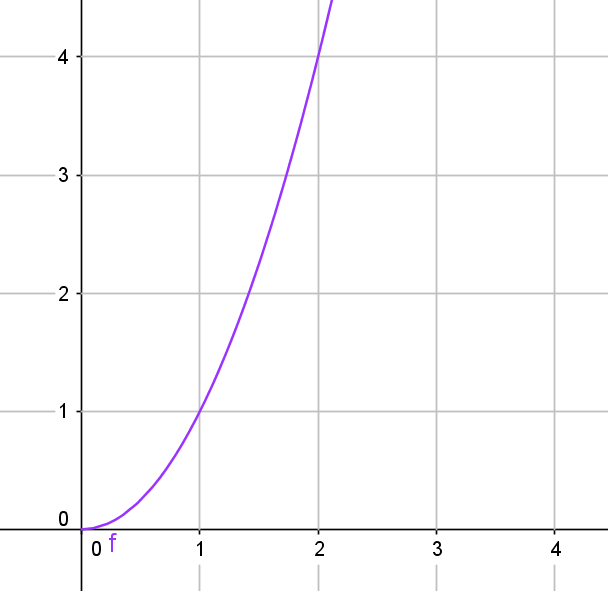
\includegraphics{irr_1_1}
\end{figure}

\noindent이므로
\(y=\sqrt x\)의 그래프는
\begin{figure}[h!]
\centering
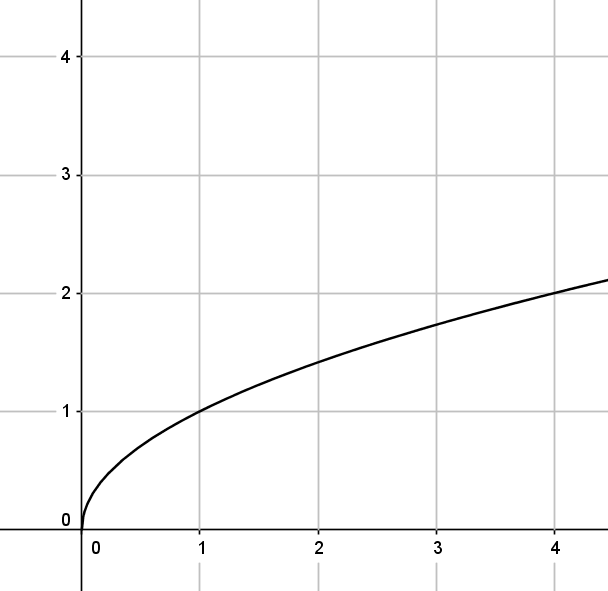
\includegraphics{irr_1_2}
\end{figure}

\noindent이다.

\clearpage
%%
\subsection{\(y=\pm\sqrt{ax}\)}

%
\exam{\(y=\sqrt{2x}\)}
\(y=\sqrt{2x}\)의 그래프를 그려보자.
이 식은 \(y=\sqrt2\sqrt x\)라고 쓸 수 있으므로 \(y=\sqrt x\)의 그래프를 세로 방향으로 \(\sqrt2\)배만큼 늘리면 \(y=\sqrt{2x}\)의 그래프가 된다.
\(x=2\)일 때, \(y=2\)이므로 \((2,2)\)를 지나도록 그래프를 그리면 아래와 같다.
\begin{figure}[h!]
\centering
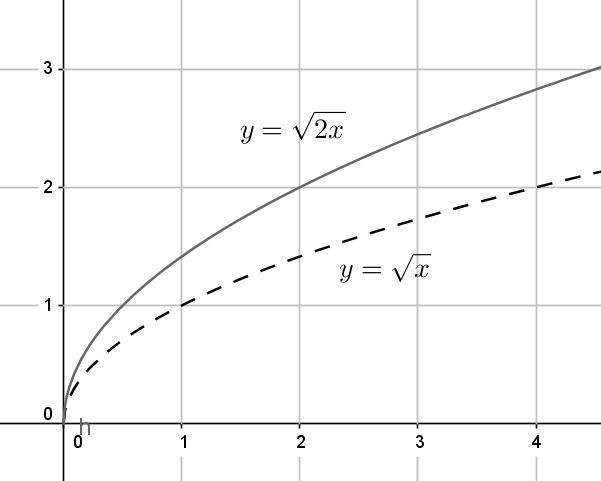
\includegraphics{irr_2_1}
\end{figure}

%
\exam{\(y=\sqrt{-x}\)}
\(y=\sqrt{-x}\)의 그래프를 그려보자.
이 식은 \(y=\sqrt x\)에서 \(x\) 대신 \(-x\)를 대입해서 얻어지므로 \(y=\sqrt x\)의 그래프를 \(y\)축을 중심으로 대칭이동시켜 그릴 수 있다.
\begin{figure}[h!]
\centering
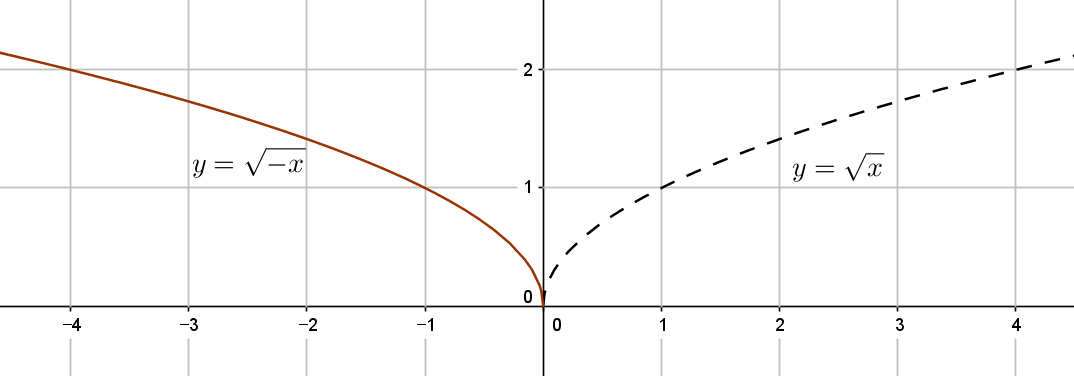
\includegraphics{irr_2_2}
\end{figure}

\clearpage
%
\prob{\(y=\sqrt{3x}\)}
\(y=\sqrt{3x}\)의 그래프를 그려보자.
이 식은 \(y=\sqrt3\sqrt x\)라고 쓸 수 있으므로 \(y=\sqrt x\)의 그래프를 세로 방향으로 \(\sqrt3\)배만큼 늘리면 \(y=\sqrt{3x}\)의 그래프가 된다.
\(x=3\)일 때, \(y=\pb{3}\)이므로 \((\pb{3},\pb{3})\)를 지나도록 그래프를 그리면 아래와 같다.

\begin{figure}[h!]
\centering
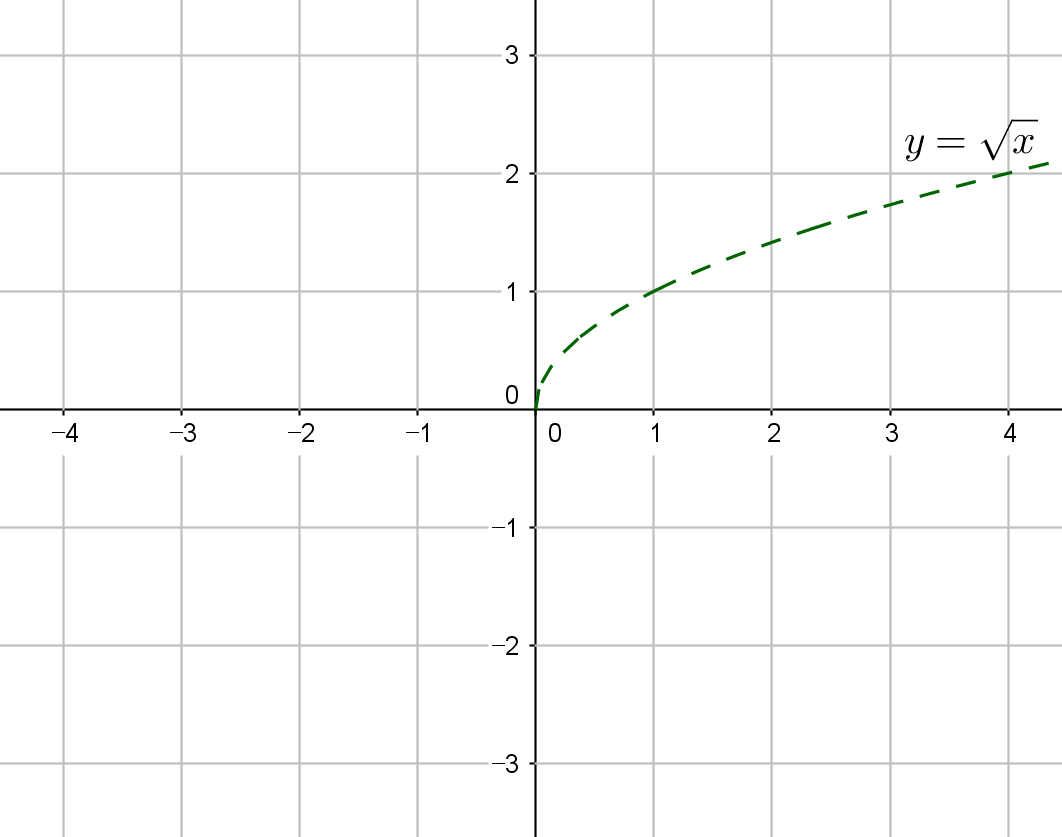
\includegraphics[width=0.63\textwidth]{irr_2_3}
\end{figure}

%
\prob{\(y=\sqrt{\frac12x}\)}
\(y=\sqrt{\frac12x}\)의 그래프를 그려보자.
이 식은 \(y=\frac1{\sqrt2}\sqrt x\)라고 쓸 수 있으므로 \(y=\sqrt x\)의 그래프를 세로 방향으로 \(\frac1{\sqrt2}\)배만큼 줄이면 \(y=\sqrt{\frac12x}\)의 그래프가 된다.
\(x=2\)일 때, \(y=\pb{2}\)이므로 \((\pb{2},\pb{2})\)를 지나도록 그래프를 그리면 아래와 같다.
\begin{figure}[h!]
\centering
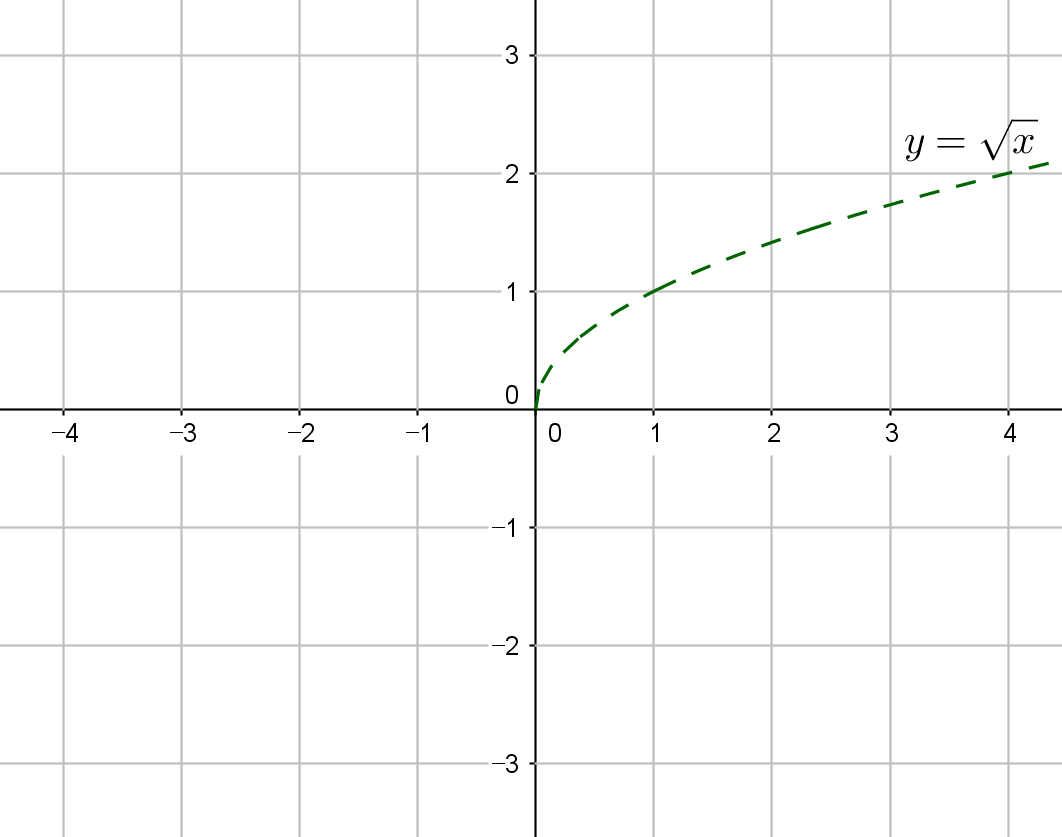
\includegraphics[width=0.63\textwidth]{irr_2_3}
\end{figure}

%
\prob{\(y=-\sqrt{x}\)}
\(y=-\sqrt{x}\)의 그래프를 그려보자.
이 식은 \(y=\sqrt x\)에서 \(y\) 대신 \(-y\)를 대입해서 얻어지므로 \(y=\sqrt x\)의 그래프를 \pb{y축}을 중심으로 대칭이동시켜 그릴 수 있다.
\begin{figure}[h!]
\centering
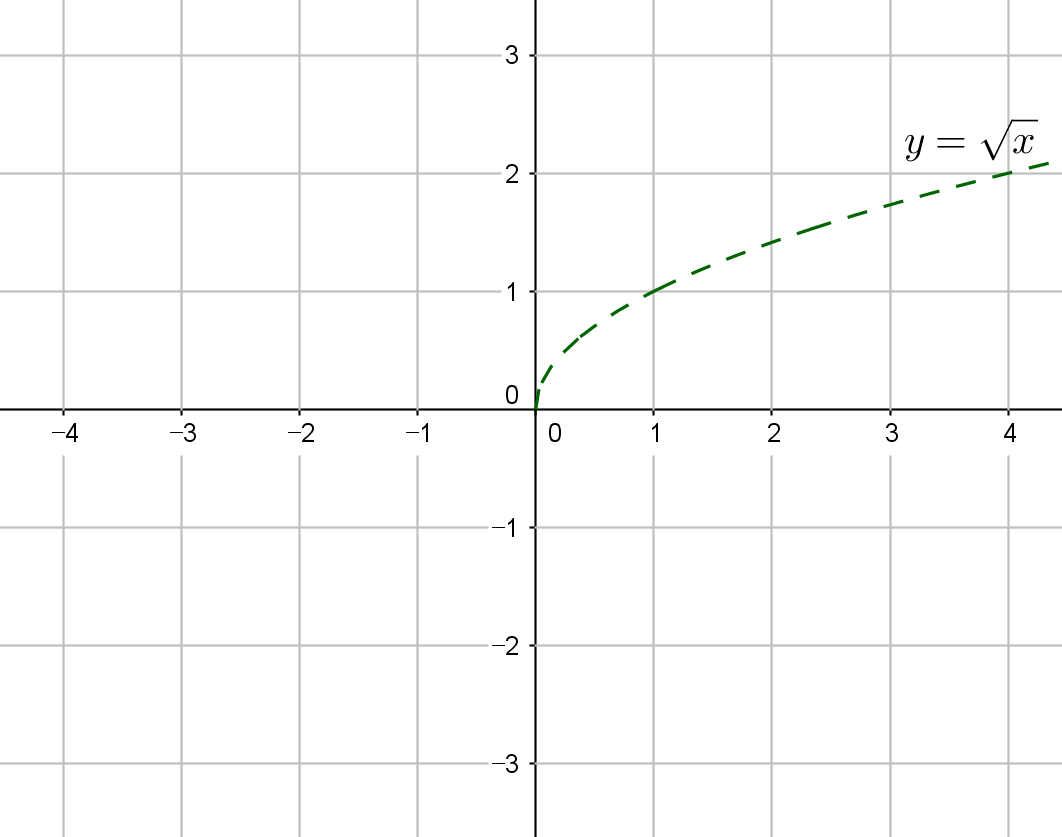
\includegraphics[width=0.65\textwidth]{irr_2_4}
\end{figure}

%
\prob{\(y=-\sqrt{-x}\)}
\(y=-\sqrt{-x}\)의 그래프를 그려보자.
이 식은 \(y=\sqrt x\)에서 \(x\) 대신 \(-x\)를, \(y\) 대신 \(-y\)를 대입해서 얻어지므로 \(y=\sqrt x\)의 그래프를 \pb{원점}을 중심으로 대칭이동시켜 그릴 수 있다.
\begin{figure}[h!]
\centering
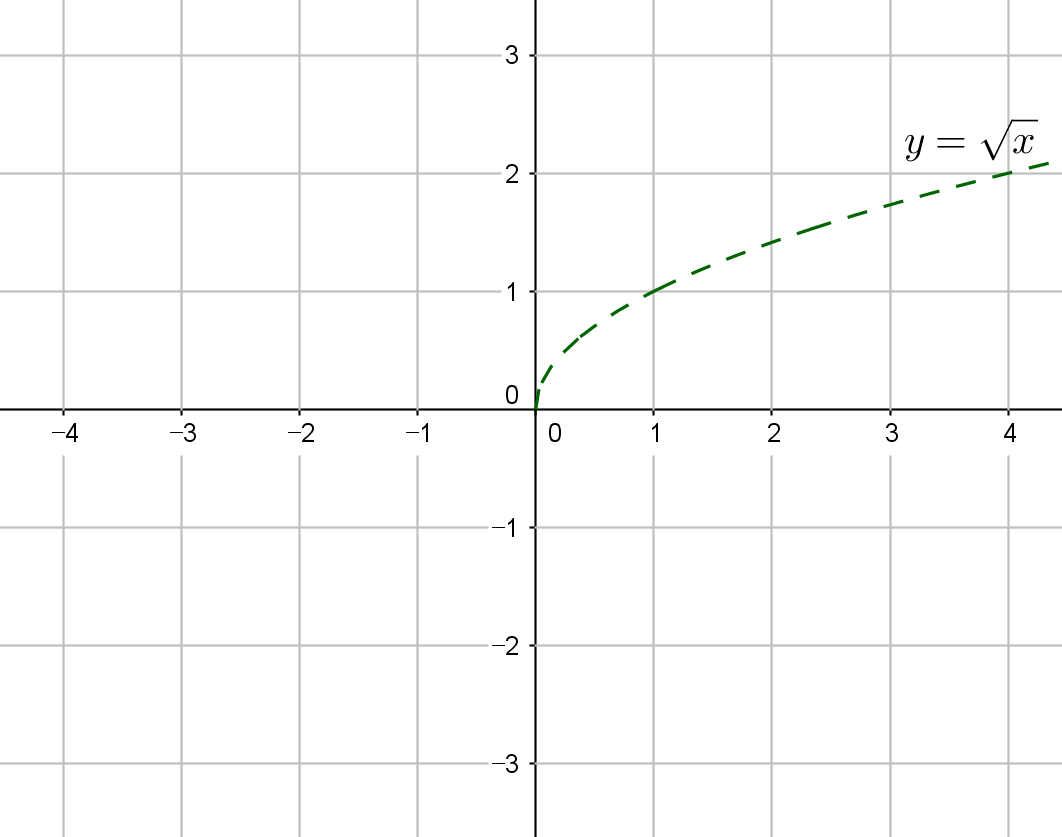
\includegraphics[width=0.65\textwidth]{irr_2_4}
\end{figure}

\clearpage

%
\prob{}
다음 식의 그래프들을 그리시오.

(1) \(y=\sqrt{4x}\)
\begin{figure}[h!]
\centering
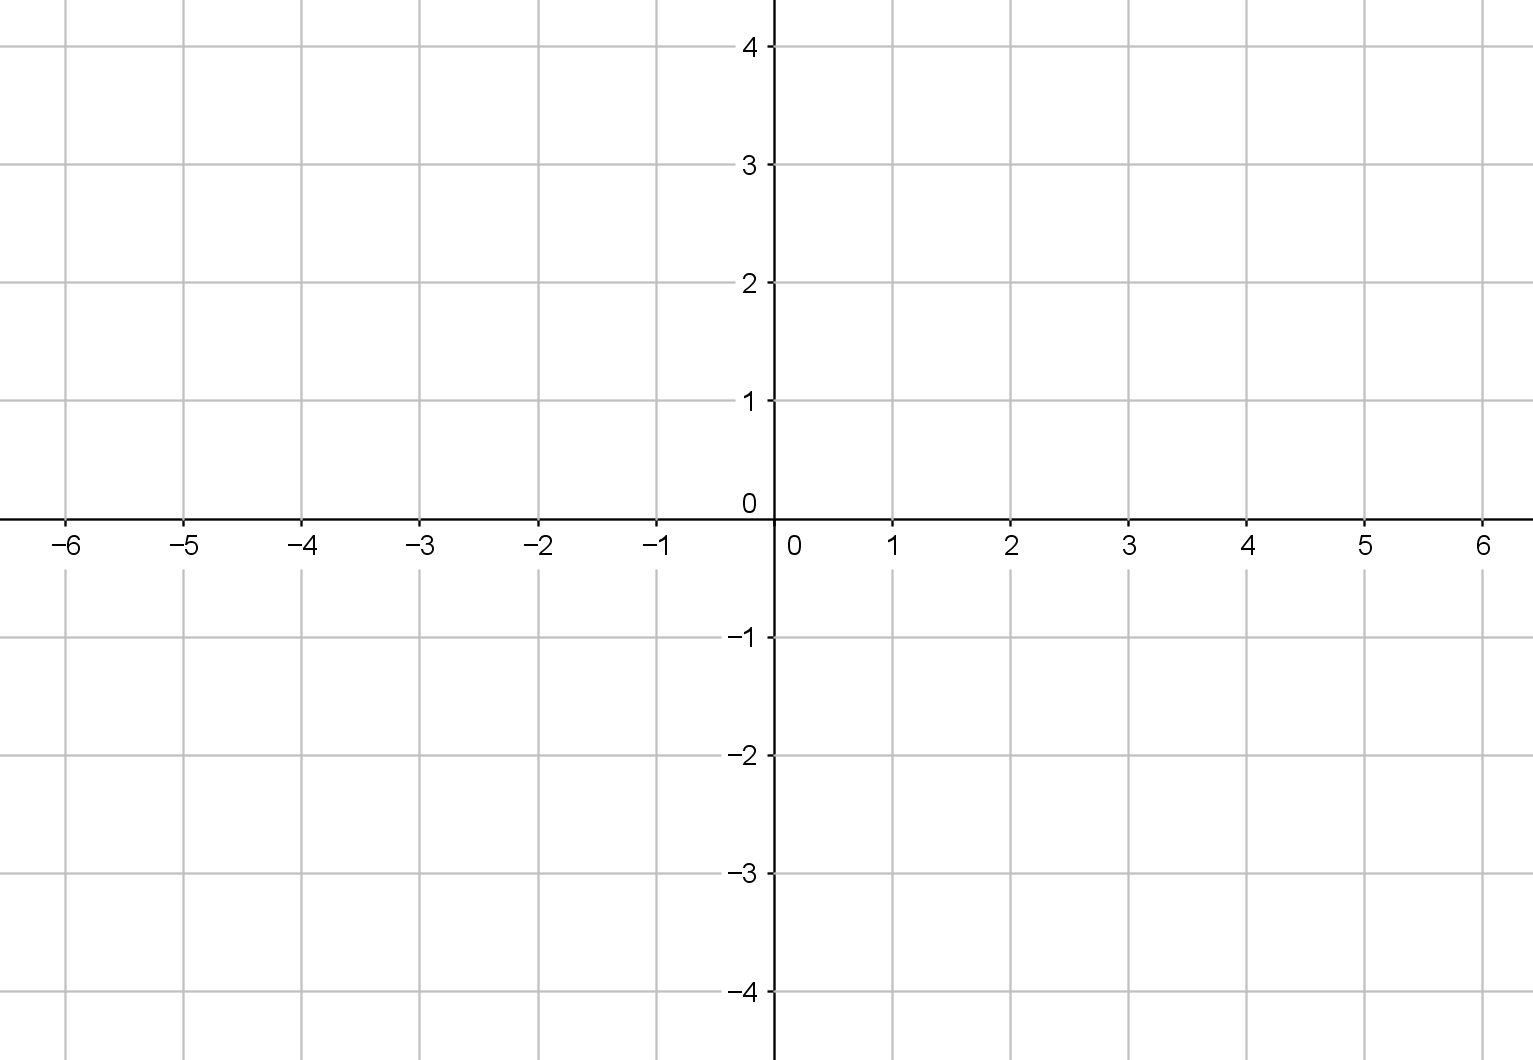
\includegraphics[width=0.9\textwidth]{irr_2_5}
\end{figure}

(2) \(y=\sqrt{\frac13x}\)
\begin{figure}[h!]
\centering
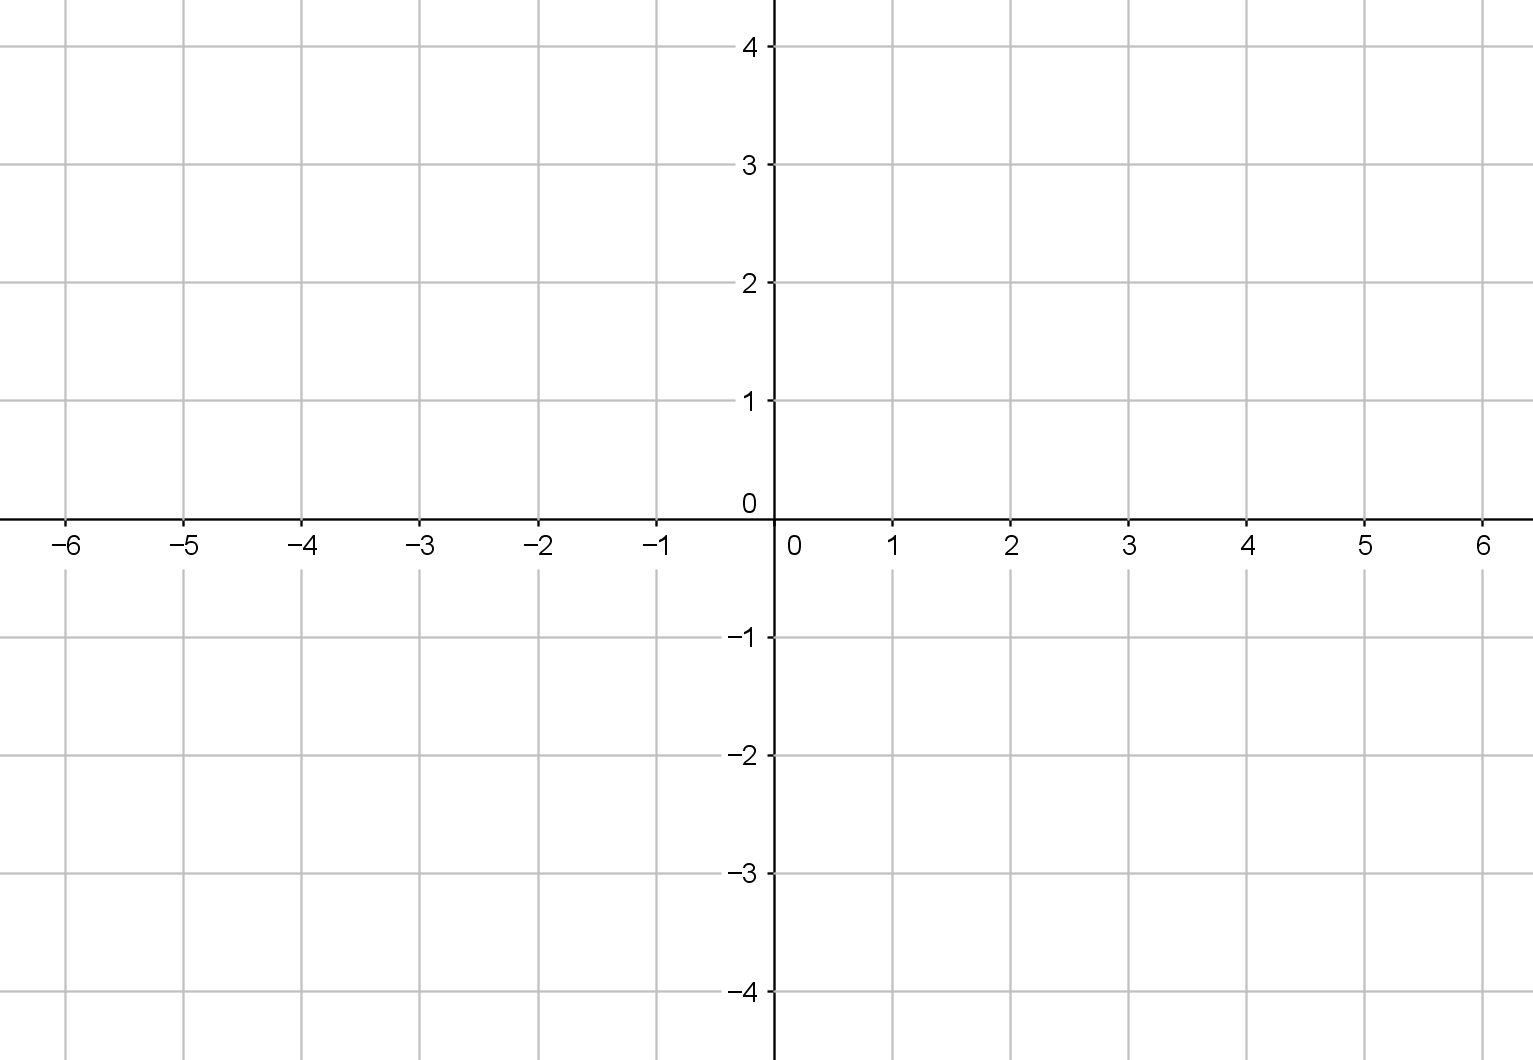
\includegraphics[width=0.9\textwidth]{irr_2_5}
\end{figure}

\clearpage
(3) \(y=\sqrt{-2x}\)
\begin{figure}[h!]
\centering
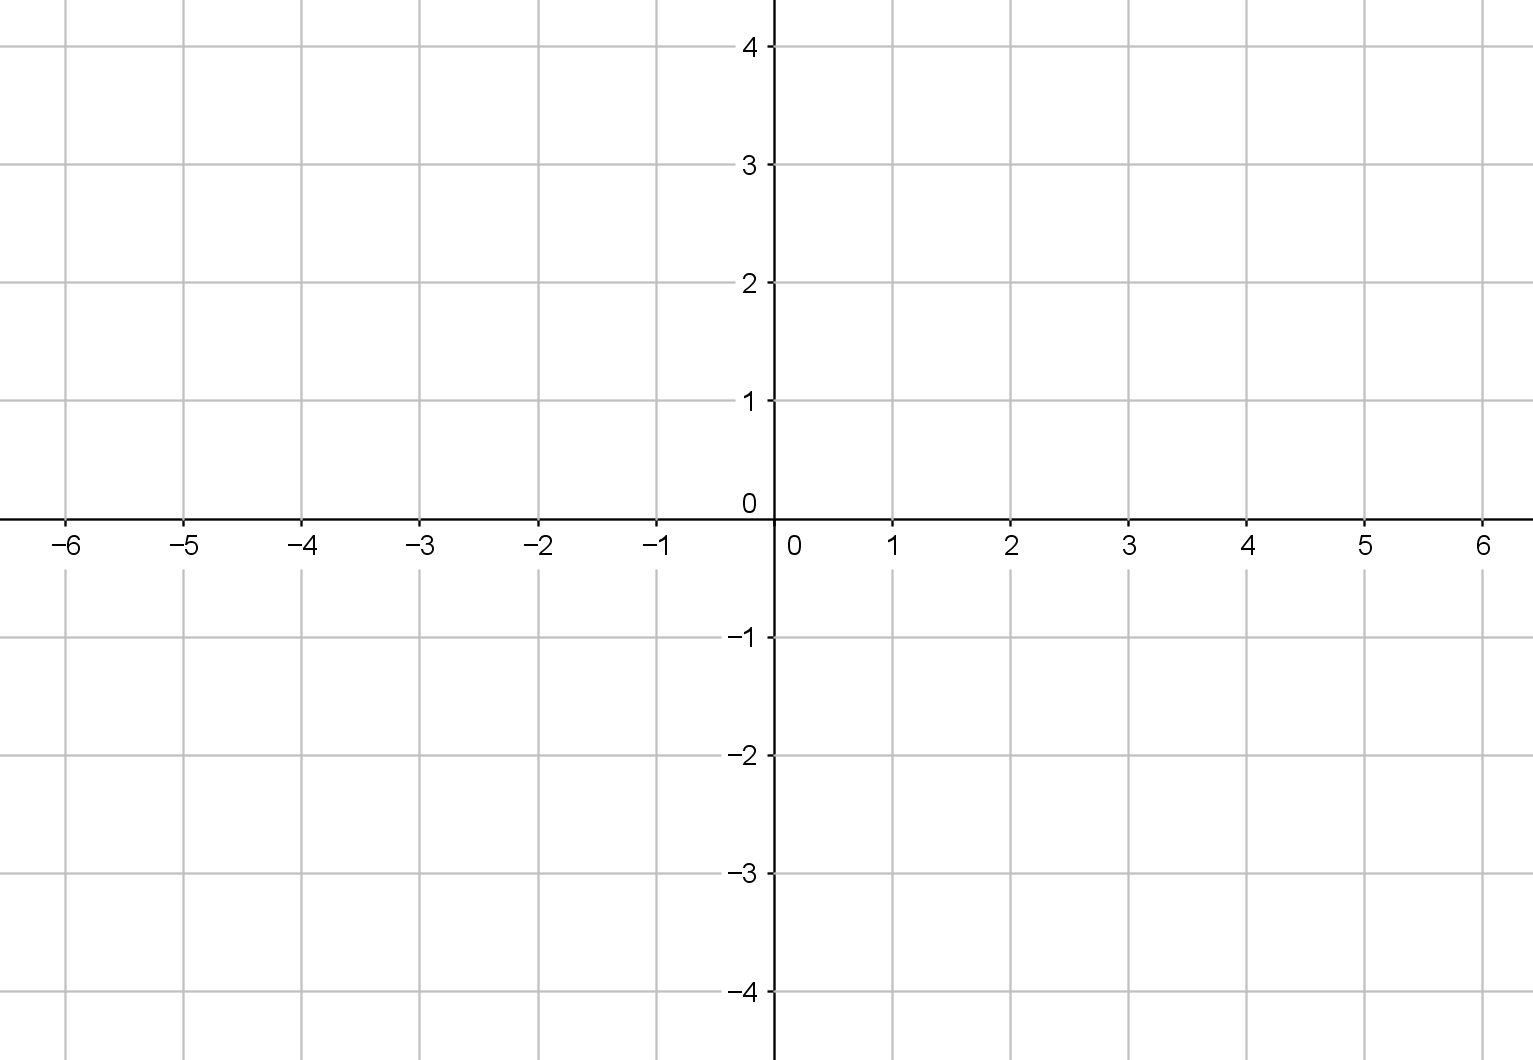
\includegraphics[width=0.9\textwidth]{irr_2_5}
\end{figure}

(4) \(y=-\sqrt{3x}\)
\begin{figure}[h!]
\centering
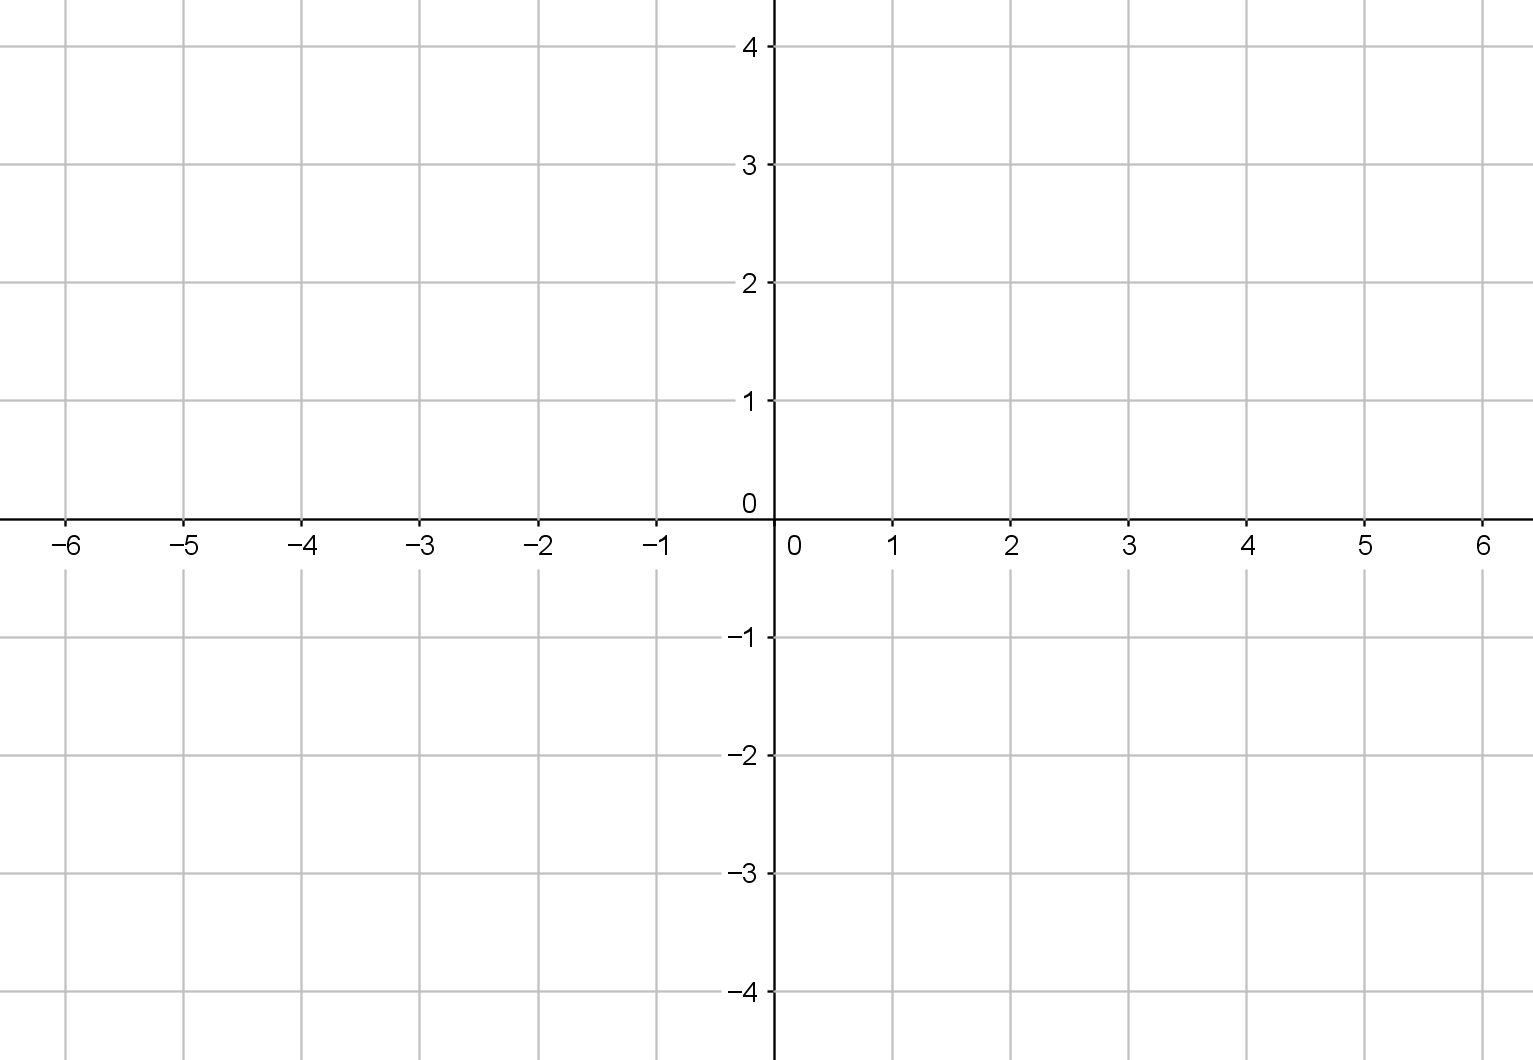
\includegraphics[width=0.9\textwidth]{irr_2_5}
\end{figure}

\clearpage
(5) \(y=-\sqrt{\frac12x}\)
\begin{figure}[h!]
\centering
\includegraphics[width=0.9\textwidth]{irr_2_5}
\end{figure}

(6) \(y=-\sqrt{-\frac32x}\)
\begin{figure}[h!]
\centering
\includegraphics[width=0.9\textwidth]{irr_2_5}
\end{figure}


\clearpage
%%
\subsection{\(y=\sqrt{a(x-p)}+q\)}

\(y=\sqrt{a(x-p)}+q\)의 그래프는 \(y=\sqrt{ax}\)의 그래프를 \(x\)축 방향으로 \(p\)만큼, \(y\)축 방향으로 \(q\)만큼 평행이동하여 얻어진다.

\begin{figure}[h!]
\centering
\includegraphics[width=0.5\textwidth]{irr_3_1}
\end{figure}

%
\exam{\(y=\sqrt{x+1}\)}
\(y=\sqrt{x+1}\)의 그래프는 \(y=\sqrt x\)의 그래프를 \(x\)축 방향으로 \(-1\)만큼 평행이동하여 얻을 수 있다.
\begin{figure}[h!]
\centering
\includegraphics[width=0.85\textwidth]{irr_3_2}
\end{figure}

\clearpage
%
\prob{\(y=\sqrt{x}+1\)}
\(y=\sqrt{x}+1\)의 그래프는 \(y=\sqrt x\)의 그래프를 \(y\)축 방향으로 \pb{-1}만큼 평행이동하여 얻을 수 있다.
\begin{figure}[h!]
\centering
\includegraphics[width=0.8\textwidth]{irr_3_3}
\end{figure}

%
\prob{\(y=\sqrt{x-2}-1\)}
\(y=\sqrt{x-2}-1\)의 그래프는 \(y=\sqrt x\)의 그래프를 \(x\)축 방향으로 \pb{2}만큼, \(y\)축 방향으로 \pb{-1}만큼 평행이동하여 얻을 수 있다.
\begin{figure}[h!]
\centering
\includegraphics[width=0.8\textwidth]{irr_3_3}
\end{figure}

\clearpage

%
\exam{\(y=-\sqrt{x+2}\)}
\(y=-\sqrt{x+2}\)의 그래프는 \(y=-\sqrt x\)의 그래프를 \(x\)축 방향으로 \(-2\)만큼 평행이동하여 얻을 수 있다.
\begin{figure}[h!]
\centering
\includegraphics[width=0.8\textwidth]{irr_3_4}
\end{figure}

%
\prob{\(y=-\sqrt{x+2}-2\)}
\(y=-\sqrt{x+2}-2\)의 그래프는 \(y=-\sqrt x\)의 그래프를 \(x\)축 방향으로 \pb{-2}만큼, \(y\)축 방향으로 \pb{-2}만큼 평행이동하여 얻을 수 있다.
\begin{figure}[h!]
\centering
\includegraphics[width=0.8\textwidth]{irr_3_5}
\end{figure}

\clearpage

%%
\subsection{\(y=\sqrt{ax+b}+c\)}
식 \(y=\sqrt{ax+b}+c\)는 \(y=\sqrt{a(x-p)}+q\)꼴로 고칠 수 있으므로 적절히 변환해 그릴 수 있다.

%
\exam{\(y=\sqrt{3x-6}\)}
\(y=\sqrt{3x-6}\)은 \(y=\sqrt{3(x-2)}\)와 같이 나타낼 수 있으므로 \(y=\sqrt{3x}\)의 그래프를 \(x\)축 방향으로 \(2\)만큼 평행이동하여 얻을 수 있다.
\begin{figure}[h!]
\centering
\includegraphics[width=0.7\textwidth]{irr_4_1}
\end{figure}

%
\exam{\(y=\sqrt{3-x}+2\)}
\(y=\sqrt{3-x}+2\)은 \(y=\sqrt{-(x-3)}+2\)와 같이 나타낼 수 있으므로 \(y=\sqrt{-x}\)의 그래프를 \(x\)축 방향으로 \(3\)만큼, \(y\)축 방향으로 \(2\)만큼 평행이동하여 얻을 수 있다.
\begin{figure}[h!]
\centering
\includegraphics[width=0.7\textwidth]{irr_4_2}
\end{figure}

%
\prob{}
다음 식의 그래프들을 그리시오.

(1) \(y=\sqrt{2x-4}+1\)
\begin{figure}[h!]
\centering
\includegraphics[width=0.85\textwidth]{irr_2_5}
\end{figure}

(2) \(y=\sqrt{-2x-4}+1\)
\begin{figure}[h!]
\centering
\includegraphics[width=0.85\textwidth]{irr_2_5}
\end{figure}

\clearpage
(3) \(y=\sqrt{3-x}-1\)
\begin{figure}[h!]
\centering
\includegraphics[width=0.85\textwidth]{irr_2_5}
\end{figure}

(4) \(y=-\sqrt{3x-3}+1\)
\begin{figure}[h!]
\centering
\includegraphics[width=0.85\textwidth]{irr_2_5}
\end{figure}


\end{document}